
\documentclass{sig-alternate-10pt}
\usepackage{url}
%\usepackage[protrusion=true,expansion=true]{microtype}  
\usepackage{graphicx} 
\usepackage{wrapfig} 
\usepackage{amsmath}
\usepackage{comment}
\usepackage{cleveref}
\usepackage{float}
\usepackage{color}
\usepackage[ruled,noend]{algorithm2e}
\usepackage{footnote}
\usepackage[font=small,labelfont=bf]{caption}

\usepackage{pifont}% http://ctan.org/pkg/pifont
\newcommand{\cmark}{\ding{51}}%
\newcommand{\xmark}{\ding{55}}%
\makesavenoteenv{tabular}
\makesavenoteenv{table}
\newcommand{\system}{\textcolor{magenta}{(MB) }}

\newcommand{\kelvin}[1]{\textcolor{blue}{(KELVIN: #1)}}
\newcommand{\amy}[1]{\textcolor{red}{(AT: #1)}}

\makeatletter


%\title{\LARGE\textbf{Rethinking How to Deploy In-Network Services}}
\title{\LARGE\textbf{Dynamic Service Chaining with \system}}


\author{\textsc{Xuan Kelvin Zou, Amy Tai, Ronaldo Ferreira, Jennifer Rexford, Pamela Zave} }

\begin{document}

\maketitle  
\begin{comment}
\begin{abstract}
In addition to delivering data efficiently, today's computer networks often perform services on the traffic in flight to provide new features, enhance security, privacy, or performance. Network administrators frequently install so-called ``middleboxes'' such as firewalls, network address translators, server load balancers, Web caches, and devices that compress or encrypt the traffic. Recent trends of Network Functions Virtualization (NFV) and Software Defined Networks (SDN) turn the network into a fungible pool of resource for running services and steering traffic. Based on a NFV setting, we propose an optimization solution. More specifically, we introduce and study a new class of multi-commodify flow problems where in addition to demands on flows and capacity constraints on edges, there is an additional requirement that flows be processed by middleboxes in the network. 

Current techniques for getting middleboxes ``on path" rely on manipulating how the network switches route traffic. However due to flow session affinity and routing policy conflicts, tweaking the routing configuration to comply with a network is clumsy and inefficient. To achieve the routing solution we obtain from the optimization scheme, we propose a middlebox-aware session protocol (MBP) that makes middleboxes an explicit part of the end-to-end path, and adds, removes or replaces middleboxes dynamically as needed. This approach is easiest to achieve in a cloud environment, where---not coincidentally--the need for scalable NFV is greatest. 
\end{abstract}

\end{comment}


 \begin{comment}
\section{Motivation}

% What do you mean by Internet can move? It sounds weird.
Today's Internet can move at any  point. The soaring demands of client
mobility  over   the  last two decades,    the   growing elasticity of
virtualized server, and the  recent trends of elastic network function
virtualiztion,   impose  new challenges   for  network  infrastructure
design.

% Change the changeable, accept the  unchangeable, and remove yourself
% from the unacceptable.--Denis Waitley

Many mobility  solutions rely on  an  artificial choke-point,  such as
name server or home agent, which  are installed as middleboxes in many
places. Recent trends of network  function virtualization aim to offer
a more scalable and flexible middlebox functions, and network function
migration can happen at any  time. We raise  a question, can we have a
unified solution that can support every point (e.g., endhosts, network
functions, server VMs) moving in the network?

Although previous approaches consider some of  the problem we address,
none addresses all this issues in a unifying solution.

\end{comment}
 
%%%%%%%%%%%%%%%%%%%%%%%%%%
%%%%%INTRODUCTION
%%%%%%%%%%%%%%%%%%%%%%%%%%

\section{Introduction}

\textit{Middleboxes    are   ubiquitous     and   elastic}:    Network
administrators   use middleboxes to     apply services on the  traffic
exchanged  between pairs of  communicating  endpoints. Today, they are
routinely  used   to improve  security   (firewall,  packet scrubber),
protect  user privacy (encryption,  anonymization),  share a set of IP
addresses (network address  translator), spread traffic over  multiple
backend  servers  (load   balancing),   reduce  bandwidth  consumption
(compression, video transcoding, caching), monitor traffic and perform
application-specific    tasks.   Recent trends   of network   function
virtualization (NFV) implement   middleboxes  as virtual  machines (VMs)  or
user-space  applications separate     from   the  physical      host.
Virtualization enables running network functions (NFs) at many different locations
in the  network or even in public  clouds, and the  NF instance
can spin up (or down) or even migrate as load demands.

%, Internet of things such as connected  cars over the past few years 


\textit{Endpoints move}: The growing cellular network and WiFi hotspot
coverage has  pushed  the term   ``mobile''  to a   new era.  Mobility
support has  become  a   key   consideration   in terms  of    network
infrastructure  design. More and  more network applications and services  are run in
virtualized environments; the server VMs  can run anywhere and the VM
migration    can   happen at  any  moment    due   to load  balancing,
infrastructure maintenance, etc.

% \amy{As you probably know,  this paragraph is improperly placed. But
%   we can move it around later.}
To  support a new Internet  era where client  mobility, and server and
middlebox migration can take place anywhere and  anytime, we propose a
\system (definition goes here).
% that sits below an unmodified transport layer  and requires no router or  switchsupport. The core of  the architecture  is  a new geomorphic view of today's  network.  

The  existence  of middleboxes  already  breaks the
end-to-end principle, so we capitalize  on this violation to create  a
new  abstraction for a connection.  We  identify  each connection by a
supersession and  a list  of   subsessions, where  a   supersession
represents  the original  end-to-end communication. NF  traffic
steering simply stitches  the subsessions together, and  mobility and
migration apply the  same  building block  operation:  replacing an old
subsession with a new  one. Hence, the subsession abstraction exists
to   isolate  middlebox operations in   a  supersession to individual
subsessions.  



% \amy{This concluding  sentence is a bit  awkward-- I  don't know the
%   convention for this.}.

Although previous works consider some of the problems we address, none
provides  a  comprehensive  solution  for   endpoint  mobility, server
migration    and  middlebox  service     chain  and  migrations.   TCP
Migrate~\cite{TCPMobile}, Mobile IP~\cite{mip},   Serval~\cite{serval}
and ROAM~\cite{I3Mobile}  support endpoint mobility,  but none of them
explicitly deals  with the existence  of middleboxes. DoA~\cite{DOA} proposes a delegation architecture
for   middlebox  service  chain,   however  it  neither  supports flow
migration     across     NF       nor    server    migration.
SIMPLE~\cite{SIMPLE} and OpenNF~\cite{OpenNF} take advantage of modern
switches that offer fine-grained control  over routing (e.g., OpenFlow
enabled  switch),  to steer traffic selectively  through  one  or more
middleboxes.  However, the  routing solutions fail to support endpoint
mobility and  suffer from scalability  and flexibility of fine-grained
policy control due to the limited  size of ternary content-addressable
memory  (TCAM) on switches.  More  fundamentally, we argue middleboxes
should be  addressed explicitly  instead  of treated  as  second-class
citizens.

% \amy{It is unclear thus far how  you are supporting client mobility.
%   You simply  mention it in  the previous paragraph. ech, maybe this
%   discomfort will go away when you put  more in the intro. Basically
%   the previous paragraphs are awkward  because you go in depth  into
%   what your  architecture  is, but  only on  the  middlebox protocol
%   part. If  you're going to  describe things, might as well describe
%   the whole architecture and explain how  you are achieving all your
%   goals}

%In  \system middleboxes are  addressed explicitly  as the endpoints of subsessions  and  thus  can   be  an  integral  part  of  the mobility ecosystem. 

\system achieves:

\begin{itemize}
\item \textbf{Unified solution:} It  supports client mobility,  server
  migration,   middlebox  service  chain  and   flow  migration during
  middlebox migration.
\item  \textbf{Incrementally  deployable:} The system  can be deployed
  between client  and server, client   and  middleboxes, or even  just
  between middleboxes.
\item \textbf{Same socket abstraction:}  It does not change  transport
  layer,  and thus does   not require any   change to the higher-level
  application if the application is using socket abstraction.
\item  \textbf{No routing change:} Since  we  address the sub-sessions
  explicitly by the network layer, simple solutions like shortest path
  routing still work.
\item  \textbf{High performance:} An  in-kernel prototype shows that a
  shim translate layer can sustain up to 14.2 Gbps per CPU core.

% \amy{This shim translate layer just kind  of popped up out of the
%   blue. Do you think it is necessary to  mention it briefly prior
%   to this?}

\end{itemize}



%Most mobility proposals decouple IP and ID binding, by introducing an indirection point (e.g., Mobile IP~\cite{mip}), redirecting through DNS (e.g., TCP Migrate~\cite{TCPMobile}), or resolving persistent ID via a distributed hash table (DHT) (e.g.,ROAM~\cite{I3Mobile}). However, the solutions either lack the support for Middleboxes (e.g., ROAM) or requires an implicit fixed middlebox (e.g., home agent in Mobile IP). 




% However, getting middleboxes on (and off) a network path is unnecessarily complicated. Traditionally, middleboxes are dedicated appliances deployed at major juncture points, such as the gateway that connects an enterprise to the Internet. But this approach makes it difficult to apply middleboxes to internal traffic (staying within an enterprise or data center) or to use middleboxes selectively (e.g., allowing non-video traffic to bypass the transcoder).

% Two recent trends are making middlebox placement much more flexible. First, middleboxes are increasingly virtualized---implemented as virtual machines (VMs) that are separable from the physical host. This means that middleboxes can run at many different, strategic locations in the network, and the middlebox instances can spin up (or down) or even migrate as load demands. Second, modern switches offer fine-grained control over routing (e.g., using technologies like OpenFlow) to steer traffic selectively through one or more middleboxes. For example, web requests may traverse a firewall followed by a load balancer, while video traffic may traverse a firewall followed by transcoder. Together, these two trends turn the network into a fungible pool of resource for running services and steering traffic. 

\begin{comment}
\subsection{Middlebox-Aware Session Protocol}
We see  a growing number  of research papers  and industry activity on
controllers  that  perform flexible  ``traffic steering" (or ``service
chaining")  to optimize   performance  and/or  enforce policy.  Almost
exclusively, these controllers use \textit{routing} as their mechanism
of  control.  In the  worst  case, the  controller installs customized
``microflow" rules on  demand to  direct all the  packets of  each TCP
session through the chosen sequence of middleboxes. Alternatively, the
controller could proactively install  coarse-grained rules that handle
related TCP sessions in  the same way, at  the expense of less control
and greater complexity.    However, we argue  that  it  is  clumsy and
inefficient to use routing to steer different sets of sessions through
different     chains    of  middleboxes;     as    it   suffers   from
(i)\textit{scalability} and (ii)\textit{mobility}.

We argue  that middlebox-aware session protocols   (MBPs) are a better
way  to insert   and remove middleboxes  on   a path than  routing is.
Briefly, session protocols  do   not have scalability   or flexibility
problems  because the information  required  to implement each session
correctly is associated with the session itself.  For the same reason,
it  is easy to ensure session  affinity and dynamically add, remove or
swap middleboxes.  We  store  the  middlebox  policy at  a   logically
centralized policy server, which  functions like a  DNS server  or SDN
controller.   To achieve   this,  we  have to   address the  following
challenges:
%A simple comparison between MBPs and other existing systems is in Table~\ref{compare}. 

\begin{itemize}

\item \textbf{Scalable policy routing:} Due to  a limited size of flow
  table,  it is hard  to  put  in tens of    thousands to millions  of
  ``microflow" rules in to router or switches' hardware routing table.
  How to decompose  the middlebox  policies and offload   fine-grained
  policies to  end hosts and middleboxes  in an efficient way is still
  an open problem.

\item \textbf{Session affinity during flow migration:} Flows should be
  flexibly routed   between  different  middleboxes,   however,   this
  requires either maintaining a   per-session state in the  switch, or
  having complex ``time  out" rules to keep  states in the controller.
  It is important to have  a middlebox protocol which guarantees  flow
  affinity, however concurrency and  race condition make this  problem
  more challenging.

\item \textbf{Endpoint mobility   and multihoming:} Today's  end hosts
  change locations frequently due to device mobility and VM migration.
  In addition, newer  protocols   allow end devices to   use  multiple
  interfaces. We also need to address how  to seamlessly integrate end
  hosts mobility protocols and this MBP.

\end{itemize}
\end{comment}



The paper is organized as follows:
Section 2 gives motivating examples of dynamic service chaining and endhost mobility and how current solutions fail to meet the requirement. 
The architecture of \system is described in Section 3, and the protocol of supersession -- subsession establishment and migration is described in Section 4. 
Section 5 describes crucial data plane properties provided by \system. 
Implementation is described in Section 7 and evaluation in Section 7. 
Section 8 presents a discussion about deployment, security and fault tolerance. 
We cover related work in Section 9 and conclude in Section 10.   

%%%%%%%%%%%%%%%%%%%%%%%%%%
%%%%%Related work
%%%%%%%%%%%%%%%%%%%%%%%%%%
\begin{comment}
\begin{table*}[ht]\label{compare} 

\small 

\begin{tabular} {|l |c | c| c| c| c| c| c| }

\hline

                            			     &Scalable Fine-         & Supersession     & No Routing    	 &   Interdomain    &    Middlebox        &  Endpoint  &  No Application\\
						     &Grained Control        & Liveness     	& Modification  	 &   Middlebox       &Migration       &  Mobility  & change \\\hline
SIMPLE,FlowTags~\cite{SIMPLE,FLOWTAGS}        	   & $\oslash$             & $\oslash$   	& $\otimes$     	 &   $\oslash$      &    $\oslash$       &  $\otimes$   \\ \hline
OpenNF,Split/Merge~\cite{OpenNF,splitmerge}         & $\otimes$             & $\odot$     	& $\otimes$     	 &   $\oslash$      &    $\odot$         &  $\otimes$  \\ \hline
CoMB~\cite{CoMB}             & $\odot$               & $\odot$     	& $\odot$       	 &   $\otimes$        &    $\otimes$       &  $\otimes$ \\ \hline 
DoA~\cite{DOA}               & $\otimes$             & $\odot$    	 & $\odot$     	 	  &   $\odot$        &    $\otimes$       &  $\otimes$  \\ \hline
APLOMB~\cite{Aplomb}         & $\otimes$             & $\otimes$  	 & $\otimes$  	   	 &   $\odot$        &    $\odot$         &  $\otimes$ \\ \hline
Software Routing~\cite{OVS, click} & $\odot$         & $\otimes$  	 & $\odot$      	  &   $\odot$        &    $\oslash$       &  $\otimes$  \\ \hline



\end{tabular}
\caption{\small Comparison between different middlebox traffic steering solutions and mobility protocols ($\odot$ indicates that a scheme fully supports the criterion; $\otimes$ indicates a scheme does not, $\oslash$ indicates partially support or can be extended to) }
\end{table*}
\end{comment}




\section{Motivating Examples}

In this section, we first present a few scenarios where a system may require network function (NF) insertion, removal, or migration, and host mobility. We also discuss how the current solutions fail to address our requirements.


\subsection{Dynamic NF Policy}
Enterprise networks deploy various network functions for better performance and security. Being able to modify dynamically NF types/instances in a service chain improves the efficiency and flexibility of the network system. NF insertion is necessary if a flow is marked as suspicious by a coarse-grained intrusion detection and prevention system (IDPSs~\cite{IPS}) and requires a fine-grained deep packet inspection (DPI). NF removal is preferred if a connection goes through a cache proxy, but the proxy has a cache-miss and the content is uncacheable; the cache proxy may remove itself from the chain. NF load balancing is necessary if the network operators want to distribute a flow evenly among multiple instances of the same NF. Moreover, NF instance migration can happen in a network function virtualization (NFV) setting, and the flows that use the NF instance also need to migrate along with the instance. 

% \subsection{Case Study}
\begin{figure}[ht]
\centering
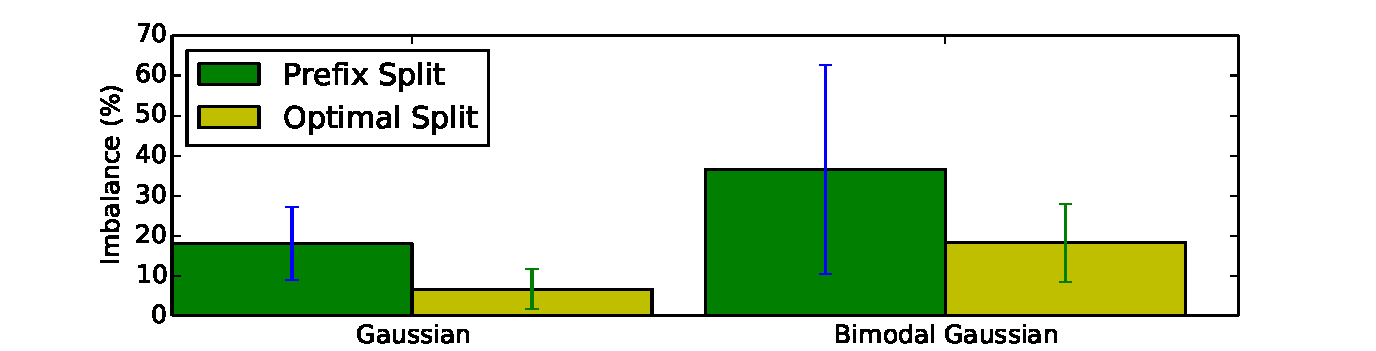
\includegraphics[width=\linewidth]{figures/routingsucks.pdf} 
\caption{\small The distribution of flow size for different prefix can be
measured using a weight\protect\cite{Niagara}. We assume two different weight
distributions for IP prefix: Gaussian, Bimodal  Gaussian with the parameters from\protect\cite{Niagara}. 
We show that in the  case of distributing flow over two  NF instances, a
routing solution, while doubling rules, fails to balance the load across middleboxes in the scenario
above. (Prefix split uses the most significant bit, and optimal split uses arbitrary one bit wildcard matching).} \label{distribution}
\end{figure}
% 


Efficient, dynamic NF policies cannot be implemented on conventional switches due to coarse-grained routing, e.g., the switch may simply tunnel all the traffic to IDS for further inspection and remove the IDS once it finds the proverbial ``needle in the haystack''. Some recent techniques leverage fine-grained routing switches (e.g., OpenFlow~\cite{openflow} based) for dynamically changing NF policies. However, these solutions are neither scalable due to TCAM rule size, nor flexible due to a complex dependency between routing rules. The SDN controller plays an excessive role in data plane, while still fails to fulfill certain network order-preserving properties~\cite{splitmerge, OpenNF}. Figure~\ref{distribution} gives an example of the imbalance caused by routing solution when trying to distribute flows across two instances of the same NF type. 

\subsection{Mobility and NF Policy} 
A cellular network can be divided into user equipment (UE), local access network (LAN) and core network.  LANs communicate to UEs through its base station and communicate to the Internet through the core network. Cellular networks rely on a wide range of NFs (e.g., firewall~\cite{IPTABLES}, load balancer~\cite{balance}, cache proxy~\cite{squid}) to improve performance and enhance security. As mobility and network function virtualization become ubiquitous, we may ask for (i) seamless mobility and (ii) dynamic service chaining.

Many mobility solutions have been proposed over the past years~\cite{mip, TCPMobile, I3Mobile, serval}, yet none of them consider the existence of network functions. Worse, NFs can even be a hindrance for these protocols since they may interfere with the protocol control logic (e.g., TCP split~\cite{TCPProxy}). Routing-based solutions have been proposed for service chaining in cellular networks(e.g., SoftCell~\cite{softcell}). However, in order to support host mobility, it places NFs only in the core network and does not support dynamic service chaining. 



%\pagebreak
\section{Architecture}\label{sec:arch}

We now  give  an overview of   \system architecture.  We  discuss  the
design goals that    motivate  a new architecture, which     separates
functionality  into three different  planes,  architecture components,
and the mechanisms to achieve the design goals.
\subsection{Design Goals}

{\bf  Scalable   policy management.}    Correctness conditions dictate that traffic must be correctly forwarded through a middlebox chain according to network policies.  Relying on routing
for traffic steering  is inefficient, because distributed
routing protocols are slow to converge during topology reconfiguration
and   provide only  coarse-grained   control  over  flows.   SDN-based
solutions  avoid this problem  by installing per-flow rules on network
switches, but these do not scale well since the SDN controller must be
involved  in per-flow decisions, and switches  have  limited memory to
store flow rules; in the worst case, each switch must install one rule
per TCP flow.

In \system,    we avoid both of    these scalability  impediments. The
protocol is designed such that the destination  address of each packet
identifies the next middlebox  or endpoint in  the path and the source
address identifies the sending  middlebox or endpoint. Doing so avoids
the need of routing tweaks  when network topology changes or endpoints
move.    Policy  management in \system  is   controlled by a logically
centralized controller,  but  packets  on the   data  plane are  never
redirected  to the policy server.   This is a  key difference from SDN
solutions  that queue packets  on the controller during flow migration
between middleboxes~\cite{OpenNF}.   Moreover, the  policy  server can
offload per-flow  decisions   to the middleboxes, for   instance allowing a
middlebox  to remove  itself  from  a session
path. Off-loading further relaxes any dependence on the policy server.

{\bf   Low  performance overhead.}   Recall    that we  identify  each
connection  with a   supersession and  its   associated subsessions. A
simple approach for decomposing a supersession into subsessions can be
implemented by establishing  tunnels between middeboxes.   However, by
adding a  new  header  to   each  packet,  this  approach   introduces  overhead   in the form of MTU  increase    and consequently  packet
fragmentation. Packet fragmentation  can  be solved by  increasing the
MTU of switches  and routers inside  a single  network administration,
but this  solution is not  viable when packets  have  to cross network
domains,  which   has become   common   in virtualized  network
functions that are outsourced to  public clouds.  Moreover,  solutions
that rely on tunnels generally add extra  overheads such as encryption
and compression~\cite{Aplomb}, features  that  can be   redundant or
unnecessary  to   all   flows.  \system   relies   on network  address
translation for explicitly  addressing subsession endpoints, hence the
only overhead is incurred by  port remapping.  Also, supersession  IDs
in \system are not carried on each  packet, as in~\cite{DOA}. They are
stored   on the   middlebox   agents  during  supersession   setup  and reconfiguration.

{\bf  Endpoint  mobility and  NF   migration.}  
%\amy{How  about  renaming    this   sub point    as   ``Separation  of 
%  Functionality'', or   something  that references the   separation of
%  decision-making into 3 planes, or  even something about  simplicity.
%  Separating planes so that  you  can cleanly implement  host mobility
%  and NF migration. In any case, the current title is meaningless.}
The growing trend in network function virtualization can cause dynamic
migration of flows between  middleboxes. Along with frequent  end host
location changes  due to device mobility  or  VM migration,  these new
possibilities  complicate     traffic-steering  solutions  relying  on
administrative control over network routing.  In \system architecture, dynamic policy changes are centrally abstracted by
a  separate policy  server, which decides  (i)   the sequence of  middleboxes
traffic should traverse and  (ii) informs the hosts --- endpoints
or  middleboxes --- of these decisions by pushing  policies ahead of time
to avoid increasing connection set-up  delay.  After fulfilling these two responsibilities, the policy server steps back  to allow  hosts to establish sessions and handle
migrations as needed.

% Incremental deployment
% This will be moved to a different subsection
% 1. Does not rely on a special  naming infrastructure. It can use any
% scheme,  as  long as   the   endpoints can   be  identified  in  the
% subsessions. A different naming scheme, however, requires applications
% and NFs changes.
% 2.  Does not require all the   components to be  integrated into the
% architecture for initial deployment. 
% 3. Does not require application or NF changes.

\subsection{Components}

An overview of  the \system architecture  with its main components and
the    interactions     between   the    modules    is    depicted  in
Figure~\ref{architecture}.   The  architecture     presents    a clear
separation of  management,  control, and  data plane functionalities.
The management  plane   is composed   of  a   policy server that    is
responsible for coordinating the agents on  the control plane based on
high-level network policies provided by the network administrator. The
control  plane implements   the protocol  in  \S\ref{sec:protocol} for
session initiation, flow migration, and network function insertion and
removal.   The data plane is  responsible for translating supersession
IDs  into local IP addresses    and ports, delivering  packets to  the
network functions,  and forwarding   packets between  middleboxes.  To
simplify  the presentation, we first  assume a homogeneous scenario in
which endpoints  and all middleboxes run \system  agents, and defer to
\S\ref{sec:discussion} a discussion of a more realistic scenario where
\system  can be deployed incrementally.  Also,  we assume that network
functions  do  not   change  the  packet  5-tuple, i.e. ---  source and
destination IP addresses  and  port numbers,  and protocol type;  the
case    where     packets  are   changed    will    be   discussed  in
\S\ref{sec:NFsupport}.

\begin{figure}[hb]
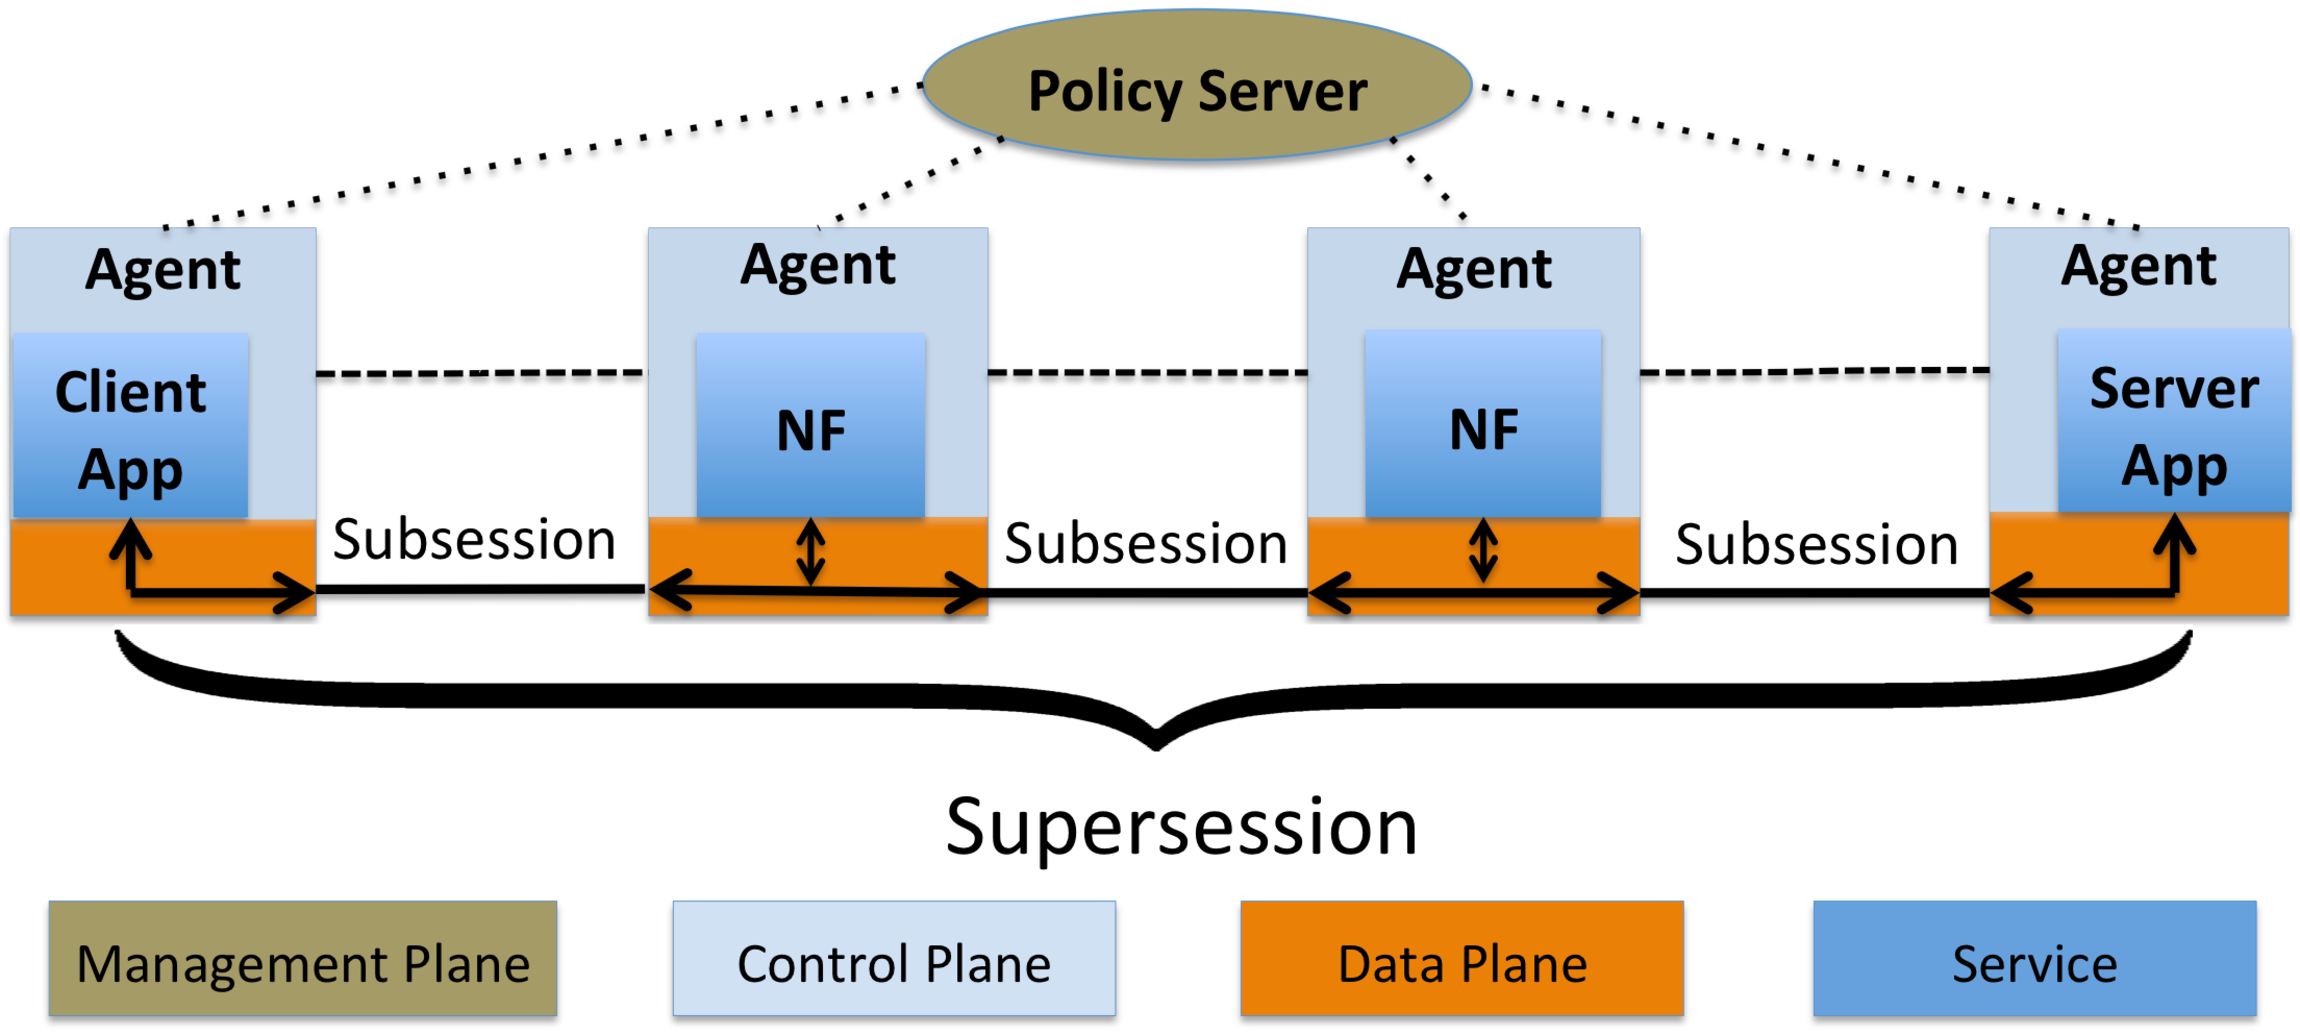
\includegraphics[width=\linewidth]{figures/archi.pdf}
\caption{\small\system architecture}\label{architecture}
\end{figure}

% Load   balancing:    Due to the    complex   packet  processing that
% middleboxes run  (e.g.,  deep packet  inspection),  a key  factor in
% middlebox deployments   is to balance the   processing load to avoid
% overload.

% To avoid inference algorithms, which  do not give 100 precision,  we
% may require  NF modifications so they  can interact with the \system
% agents.

% Typical middlebox policies require a packet (or session) to traverse
% a sequence of middlebox (This is  an instance of the broader concept
% of "service chaining").  In our example,  the administrator wants to
% route all HTTP traffic through the policy chain FW-IDS-PROXY and the
% remaining  traffic   through  the   chain FW-IDS.  Note   that  many
% middleboxes  are stateful and need to  process  both directions of a
% session for correctness.

% Middlebox resource management:  Studies show that middlebox overload
% is a  common cause of failures.  

% "The  policy server can take global   decisions to avoid overload or
% give multiple options to the \system agents  so they can balance the
% load across their neighbors.

% SIMPLE 

{\bf Policy  server:}   The  \system  policy  server is   a  logically
centralized server that receives  high-level policy specification from
the  network  administrator and reliably   delivers subpolicies to the
agents, i.e. --- it makes sure that an agent receives a policy consistent
with its location.  For instance,  a client agent should receive  only
policies related to the network it is connected.

The  policy server makes  global decisions based on: (i) configuration
changes  or (ii)   network state changes.    Configuration changes are
triggered  by the network administrator, and  network state changes are
triggered  by monitoring   information, which the  policy  server  receives  from the \system   agents. Based on the monitoring information, the policy server  may  decide to
migrate flows   from an overloaded   network function to   a different
instance, insert new network functions  in a supersession, e.g. --- introduce a DPI after  a light IDS flag packets
for deeper  inspection, or   remove a network
function  out of a  supersession path because it  is no longer needed.
To further extend system flexibility, network administrators can allow the policy server to offload decisions to the \system agents
running on the middleboxes.
A common decision that  can be easily offloaded to  the agents is  the
selection   of a     network   function instance   when  the   network
administrator configures multiple instances of the same type.

%The policy server also decides how a supersession is It determines how
%a supersession is initially divided into subsessions, i.e., it decides
%the middlebox chain a set of flows should traverse in order to enforce
%a network policy.

%- It outsources fine grain  decisions to the  middlebox agents. It can
%send to the middlebox agents a list of MB types to  from the MB chain,
%but the decision to pick an instance is outsourced to  the MBA. It can
%also provide autonomy to a MB to remove itself out the way of a flow.

In  \system,  a
policy  specifies a  predicate,  which defines a set of affected
packets, and a  sequence of network  function types.  This sequence defines the service  chain to be  traversed by the packets  satisfying the predicate, e.g. --- packets from subnet 10.0.1.0/24
should    be     forwarded       through      the     chain     \{Load
Balancer $\rightarrow$ IDS $\rightarrow$ Firewall $\rightarrow$ Proxy\}.    The general form
of a policy is:
\begin{center}
{\tt match(predicate) >> \{NFT$_1 \rightarrow\cdots\rightarrow$ NFT$_n$\}}
\end{center}
%\noindent where
%\begin{center}
%{\tt NFT$_i$ = \{Set of IP addresses\}}
%\end{center}
A predicate is specified with source and  destination IP addresses and
ports, and protocol types.   Complex predicates can be specified using
conjunction (\&),  disjunction  ($|$),  and negation (\~{})  operators
like in Pyretic~\cite{pyretic}. A packet that satisfies  the predicate in the
match  statement is forwarded  through  the chain of network  function
types specified  on the right-hand side of  the  {\tt >>} operator.  A
network   function type ({\tt NFT$_i$})   specifies  a set of  network
function instances  of the same  type. For example the network  administrator can
specify such a set of proxy servers, and
the policy  server will either choose an instance for each client or  delegate   this  decision to  the \system
agents.

%Predicates: The  predicates are specified  with respect to the point a
%packet enters  the  network,  i.e., the  point  of attachment    of an
%endpoint.


{\bf   \system Agents:} \system agents   are key enforcers of
network  policies.   They  must ensure    that  packets are  either correctly
forwarded to the next  middlebox on the  service  chain or dropped  if
they  do not   comply with  the  network policy.   Whenever  a  client
application starts a connection, the \system agent running on the same
machine intercepts the  first packet of  the connection and matches it
with  the   client's network  policies to  determine  the  sequence of
network function  types the packet must traverse.   If a match is
found, the agent  starts the session  setup protocol  in \S\ref{setup}
that   will create the     subsessions  between middleboxes  and   the
corresponding mappings as described below.   The 5-tuple of the client connection
is used to  identify the supersession  packets when they are processed
by  the  network  functions.   Once the  supersession  is   setup, all
subsequent  packets from the client's connection  are forwarded to the
first  middlebox  on  the service  chain,   and  from there  they  are
sequentially forwarded to the remaining middleboxes and to the server.

In each middlebox, a  \system agent must  create two mappings for each
session. One, which we call horizontal NAT,  translates the 5-tuple of
an incoming  packet to the corresponding 5-tuple  that is  used in the
next   subsession.  The   other one,  which   we  call vertical   NAT,
translates   the 5-tuple of each   incoming packet to the supersession
5-tuple before the  packet is delivered to the  network function or to
the applications on  the  endhosts.  Keeping the  supersession 5-tuple
invariant    on  the middleboxes  has  several advantages. First,  it
simplifies policy specification by abstracting the subsessions from the network administrator.  Second,  it simplifies network function state
migration, because network functions  always receive packets  with the
supersession  5-tuple   regardless of flow    migrations or  middlebox
insertions  or removals.  Third,  network functions that do not change
the packet 5-tuple do not need to be changed to work with \system.

\system agents are also heavily involved  in service chain maintenance
and  supersession  reconfigurations.   The  agents report   management
information, such as resource utilization  in the middleboxes, to  the
policy server, so  it  can  make  global management  decisions   about
service chains.  If allowed by network policy, reconfigurations can  also be triggered by a  network
function.   A  common case  of a
reconfiguration triggered by a network function is  when a cache proxy
detects that the content of a session is not cacheable and signals the
\system agent to  remove the  proxy  from the service  chain.  Once  a
reconfiguration is  initiated, either by the policy   server or by the
network function,  \system      agents  execute the  protocols      in
\S\ref{MigrateLogic}.

%{\bf End hosts:}

%\subsection{Division of Labor}

%Clean separation of control, data, and management 

%\subsection{Mechanisms}




% archiIllustrrate
\begin{comment}
\begin{figure}[hb]
\centering
% 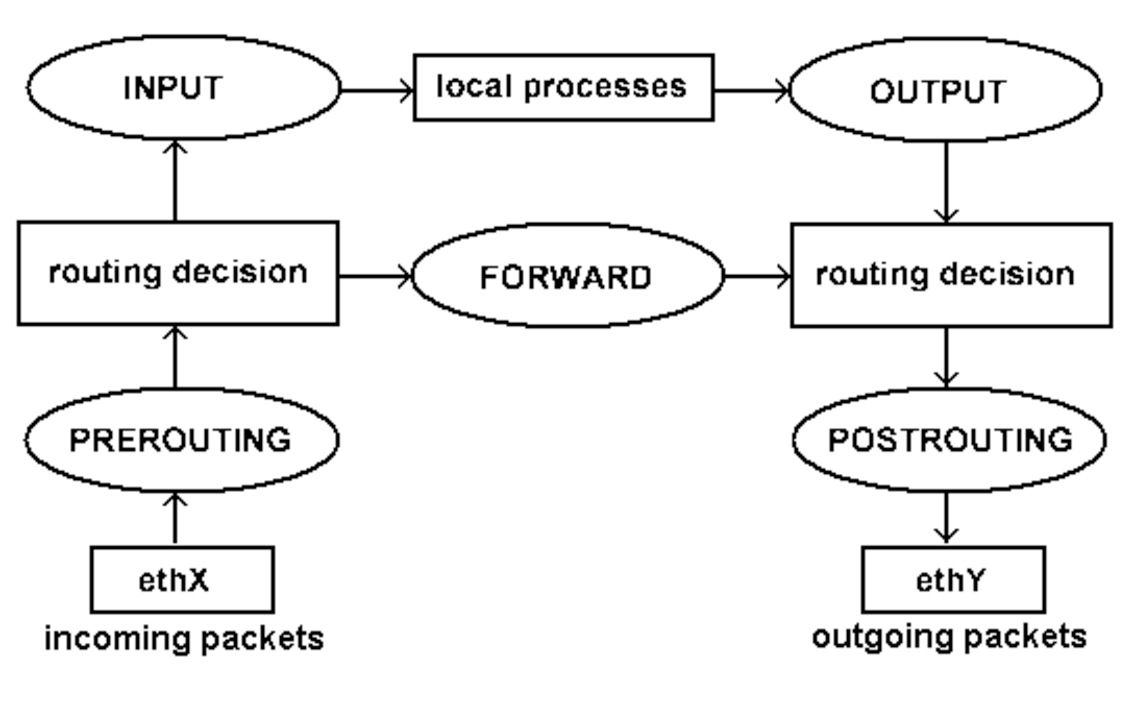
\includegraphics[scale=0.25]{figures/netfilter.pdf} 
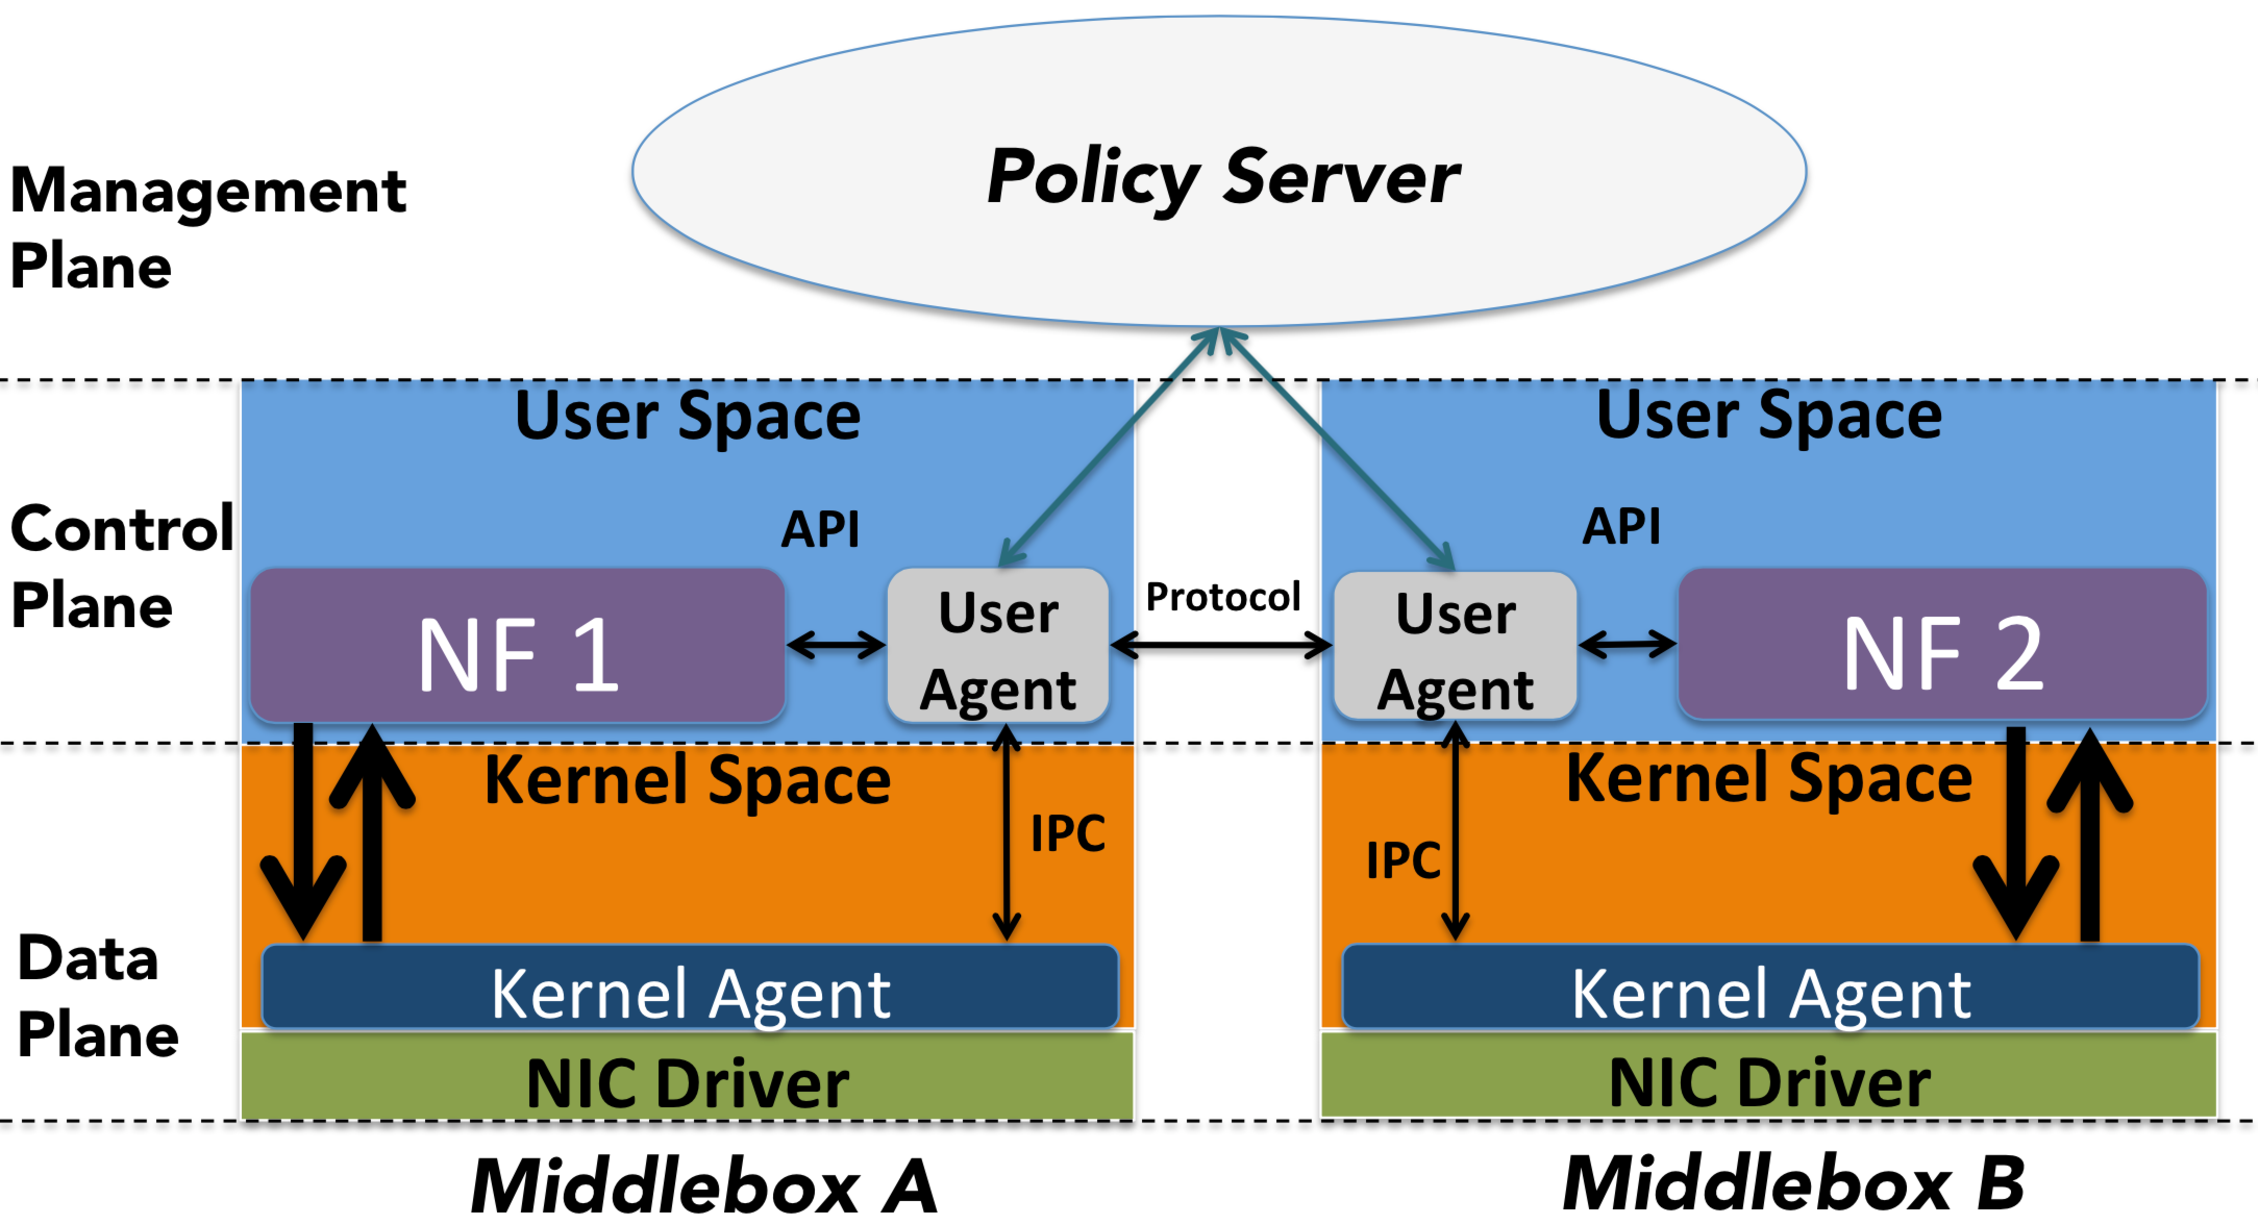
\includegraphics[width=\linewidth]{figures/archiIllustrrate.pdf} 

\caption{\small Middlebox protocol architecture}\label{expTopo}
\end{figure}
\end{comment}

\section{Protocol}
\label{sec:protocol}
\begin{comment}
We explain the basic indirection protocol in subsection~\ref{basic}, a three-way handshake that exchanges state enabling future migration in subsection~\ref{twoway}, and a migration protocol in subsection~\ref{mobile}. The middlebox-aware session protocol can: (i) successfully establish a connection through the two-way handshake; (ii) support a flexible migration of either endhosts or middleboxes; and (iii) gracefully close the connection, or sub-sessions during the migration. 
\end{comment}

Considering middleboxes as explicit components of the end-to-end between two endpoints is the crux of our protocol. Only by doing so can we achieve the desired scalability and flexibility for both endpoints and middleboxes. We discuss session setup in \S\ref{setup} and flow migration control in \S\ref{MigrateLogic}.  

\subsection{Session Setup}\label{setup}

In \system protocol, each endpoint or middlebox sends packets whose destination is the next middlebox or endpoint in the session path. This obviates the need for special support in the switch or router to direct packets through the chosen chain of network functions (service chain), despite changes in network topology or host movement. 

The list of middleboxes, $L$, that a flow has to traverse is provided by the policy server and can be pulled from the server or pushed to the client. When the client initiates the connection, the control plane uses a three-way handshake to establish the supersession and its associated subsessions. More specifically, the client's control plane sends a SYN message that includes the supersession header and $L$ to the first middlebox. The middlebox strips itself from the head of $L$, gets the address of the next middlebox from $L$, and relays the rest of the message to the next middlebox. The SYN message is thus passed recursively through the elements of $L$ before reaching the server. Upon receiving the SYN, the server sends a SYNACK back to the client along $reverse(L)$. Upon receiving the SYNACK, the client immediately sends an ACK to the server via the same mechanism. Once these three control messages are exchanged, the supersession and subsessions are established, and data packets are explicitly addressed to the subsession IPs.

If we simply rewrite the source and destination IPs as described in our ``horizontal NAT'', we lose supersession information and introduce ambiguity. Consider the case where flow \textit{a} and \textit{b} have the same source port and destination IP and port, but different source IPs. If \textit{a} and \textit{b} share the same first hop middlebox, the two flows may become indistinguishable upon arrival at the first hop middlebox. To address this issue, we modify the port numbers to identify the flow, a standard technique in NAT~\cite{NAT}. We integrate this port allocation into the three-way handshake: when a middlebox receives a SYN, it assigns port mappings and initiates the next subsession with the rewritten port numbers. If we rewrite both source and destination ports, \system can support four billion unique flows per middlebox pair. See Figure~\ref{sessionsetup} for the complete session setup. \amy{ Can we insert some words over the port remapping in Figure 3, to indicate that the $\rightarrow$ represents port remapping?}

\begin{figure}[ht]
\centering
% 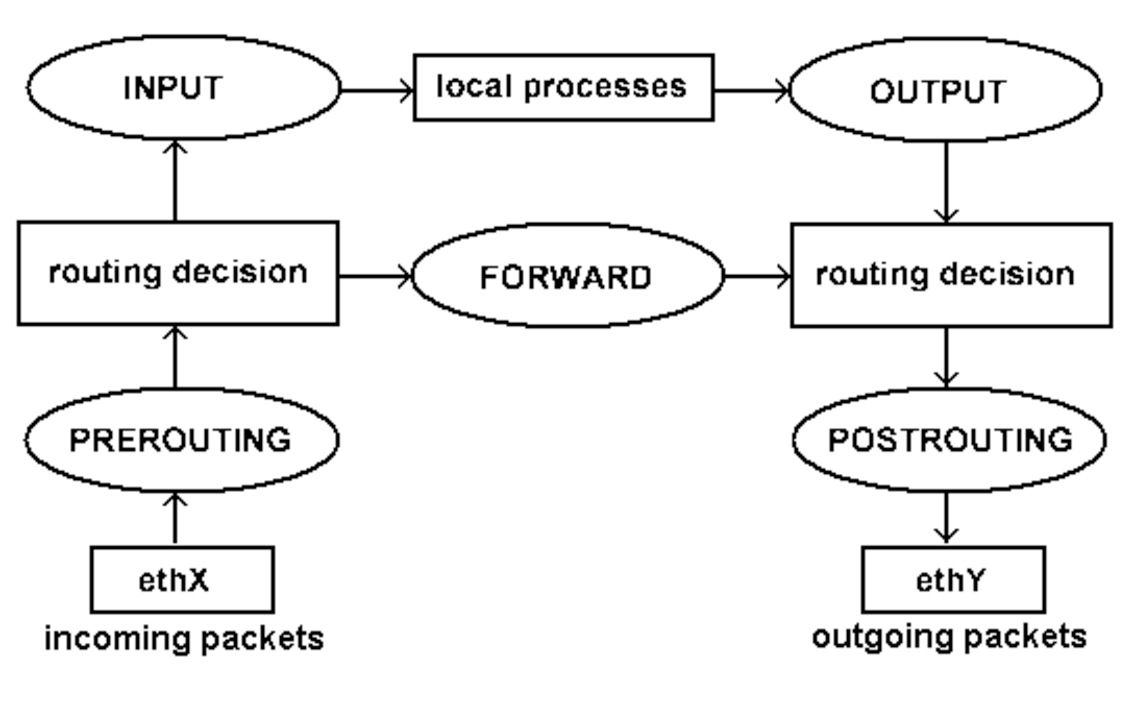
\includegraphics[scale=0.25]{figures/netfilter.pdf} 
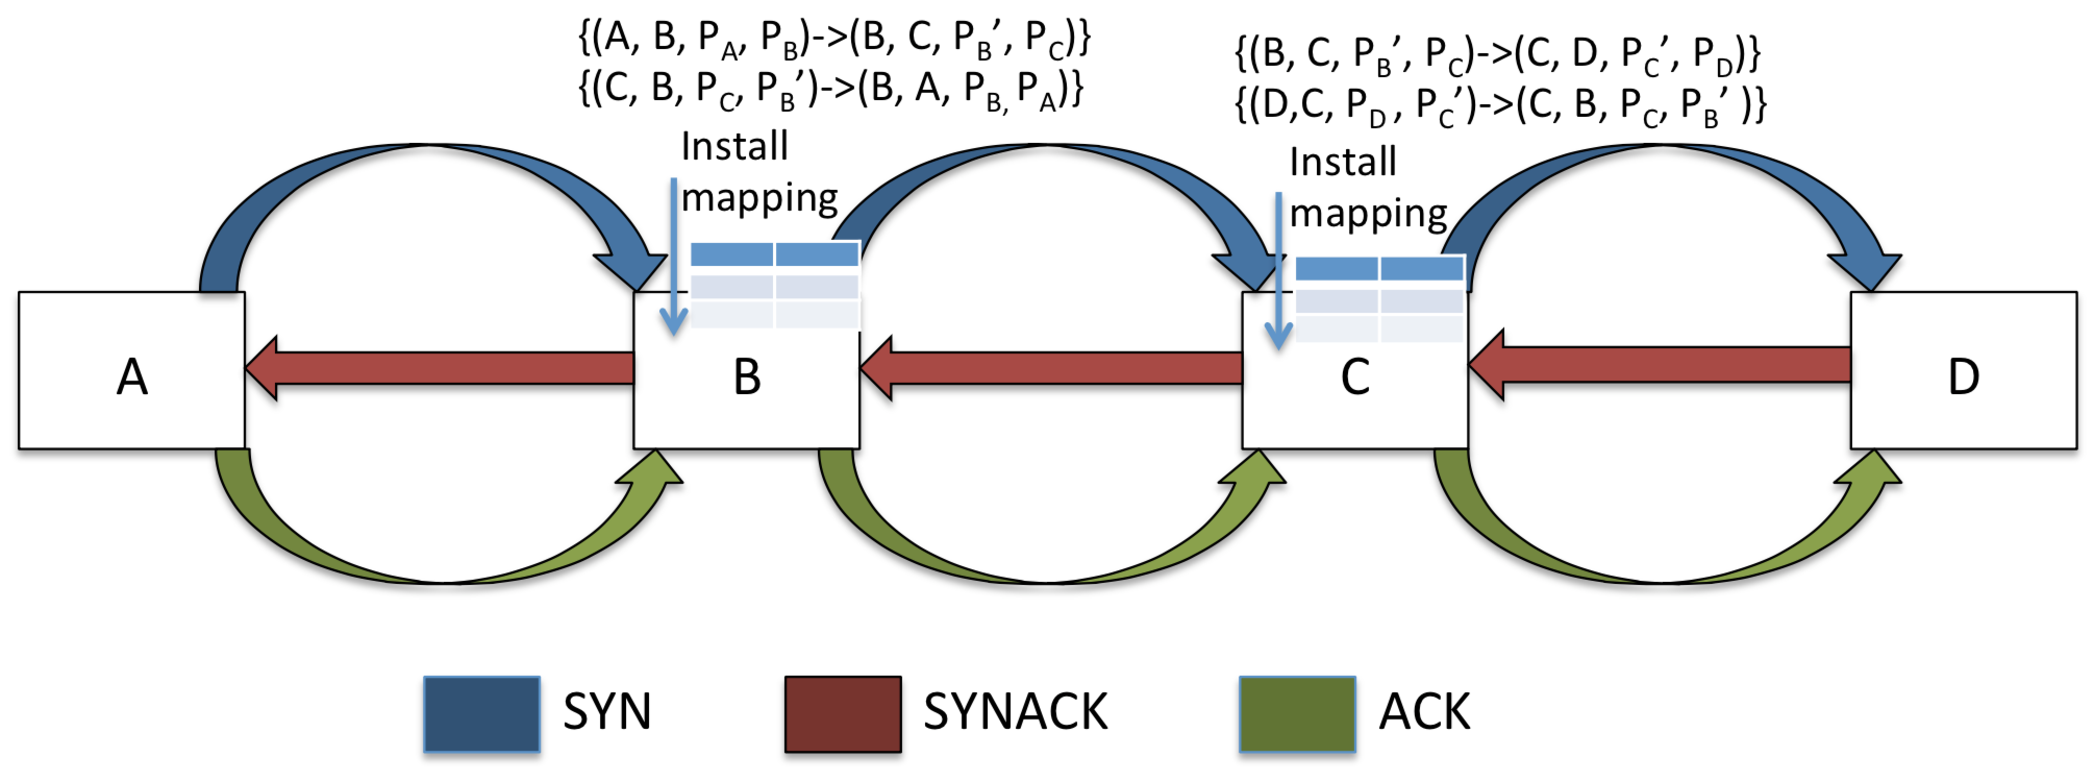
\includegraphics[width=\linewidth]{figures/threeway.pdf} 

\caption{\small  Session setup}\label{sessionsetup}
\end{figure}



\subsection{Migration and Mobility Control}\label{MigrateLogic}
%Dynamic network function policies are gaining ground today because of the flexibility they offer. 

Supporting dynamic middlebox modification for a flow improves the efficiency of the network and NF use, e.g. --- removing a cache proxy if the content is not cache-able, inserting an IDS upon detecting suspicious flows, or switching from a heavily loaded transcoder to a lightly loaded one. As a natural extension of general middlebox migration, we include endhost mobility in the design of \system; supporting mobility is also critical in cellular networks.

\subsubsection{``Make before break''} \label{migration1}
To find the right mechanism to support flow migration, we investigated existing mobility protocols~\cite{TCPMobile, I3Mobile, mip, serval, lisp, hip} under the session-location mobility framework~\cite{zave}. However, the key distinction between host mobility and NF flow migration is that a move in host mobility is unexpected, whereas flow migration among middleboxes is planned.

In fact, this type of reconfiguration is quite common in circuit design and addressed via the ``make before break'' philosophy. Namely, we stitch together subsessions on the new path before closing the subsessions on the old path. To achieve this, we treat the two neighbors of the moving middlebox as two \textit{signaling endpoints} during a flow migration. We stress that the resulting three nodes that are involved in the migration are \textit{consecutive}. Because we offload some policy decisions to the middleboxes, this property ensures that a middlebox cannot decide the fate of other on-path middleboxes that are not directly affected by the migration. 

For middlebox insertion, we first deterministically identify and notify one of the two signaling endpoints as an initiating point. Starting at the initiating point, we set the two signaling endpoints to a suspend state to prevent data transfer on the new path and complete a three-way handshake (UPDATE-SYN, UPDATE-SYNACK and UPDATE-ACK) on the new path, consisting of the two signaling endpoints and the new middlebox. Once the new path is established, we commence data transfer on the new path and remove the old path. We extend the same mechanism to handle middlebox removal and replacement. 

\subsubsection{Handling Concurrent Migration}
For correctness, we must properly deal with cases where two middleboxes initiate simultaneous move operations. In particular, if two neighbor middleboxes both initiate removal, we may lose the supersession connection. Strawman solutions include: (1) using a two phase commit to allow the one with the highest ID to move first; (2) a central controller that assigns token to the middleboxes. However, strong serialization via a two phase commit is not necessary, and a central controller suffers from scalability, one of our initial design goals.

To address concurrent migration, we rely on the following properties: (i) migration is per flow, and (ii) at most three nodes on the current service chain are involved in each flow migration. The two assumptions help us design an efficient algorithm in which migration can happen simultaneously for different flows, and concurrent migrations can happen at different points of the service chain if they involve disjoint sets of nodes; each node has a \texttt{pending} counter to ensure that it participates in at most one concurrent update.


The proposed algorithm only allows one concurrent operation for all the nodes involved. When a migration is initiated at a certain node, the node postpones the update if its \texttt{pending} counter is not zero. Otherwise it increments the \texttt{pending} counter and sends the request to the node immediately to its left if the migration is removal or replacement, or connects to the new middlebox if it is an insertion. Middleboxes for a flow have a strict ordering, which is simply the order in which the middleboxes are traversed by the path from the client to the server. We define two comparators on this ordering, which we term ``left'' and ``right''. $M_{1}$ is left of $M_{2}$ iff the path from the client to $M_{2}$ passes through $M_{1}$; $M_{1}$ is right of $M_{2}$ iff the path from the client to $M_{1}$ passes through $M_{2}$. If the left node responds with a reject, the node backs off, otherwise it receives an approval and proceeds with the update. A node always accepts UPDATE-SYN requests to establish a new path. Algorithm~\ref{concurrency} describes the algorithm details and Figure~\ref{concurfigure} depicts the steps for migrations.


\begin{figure}[ht]
\centering
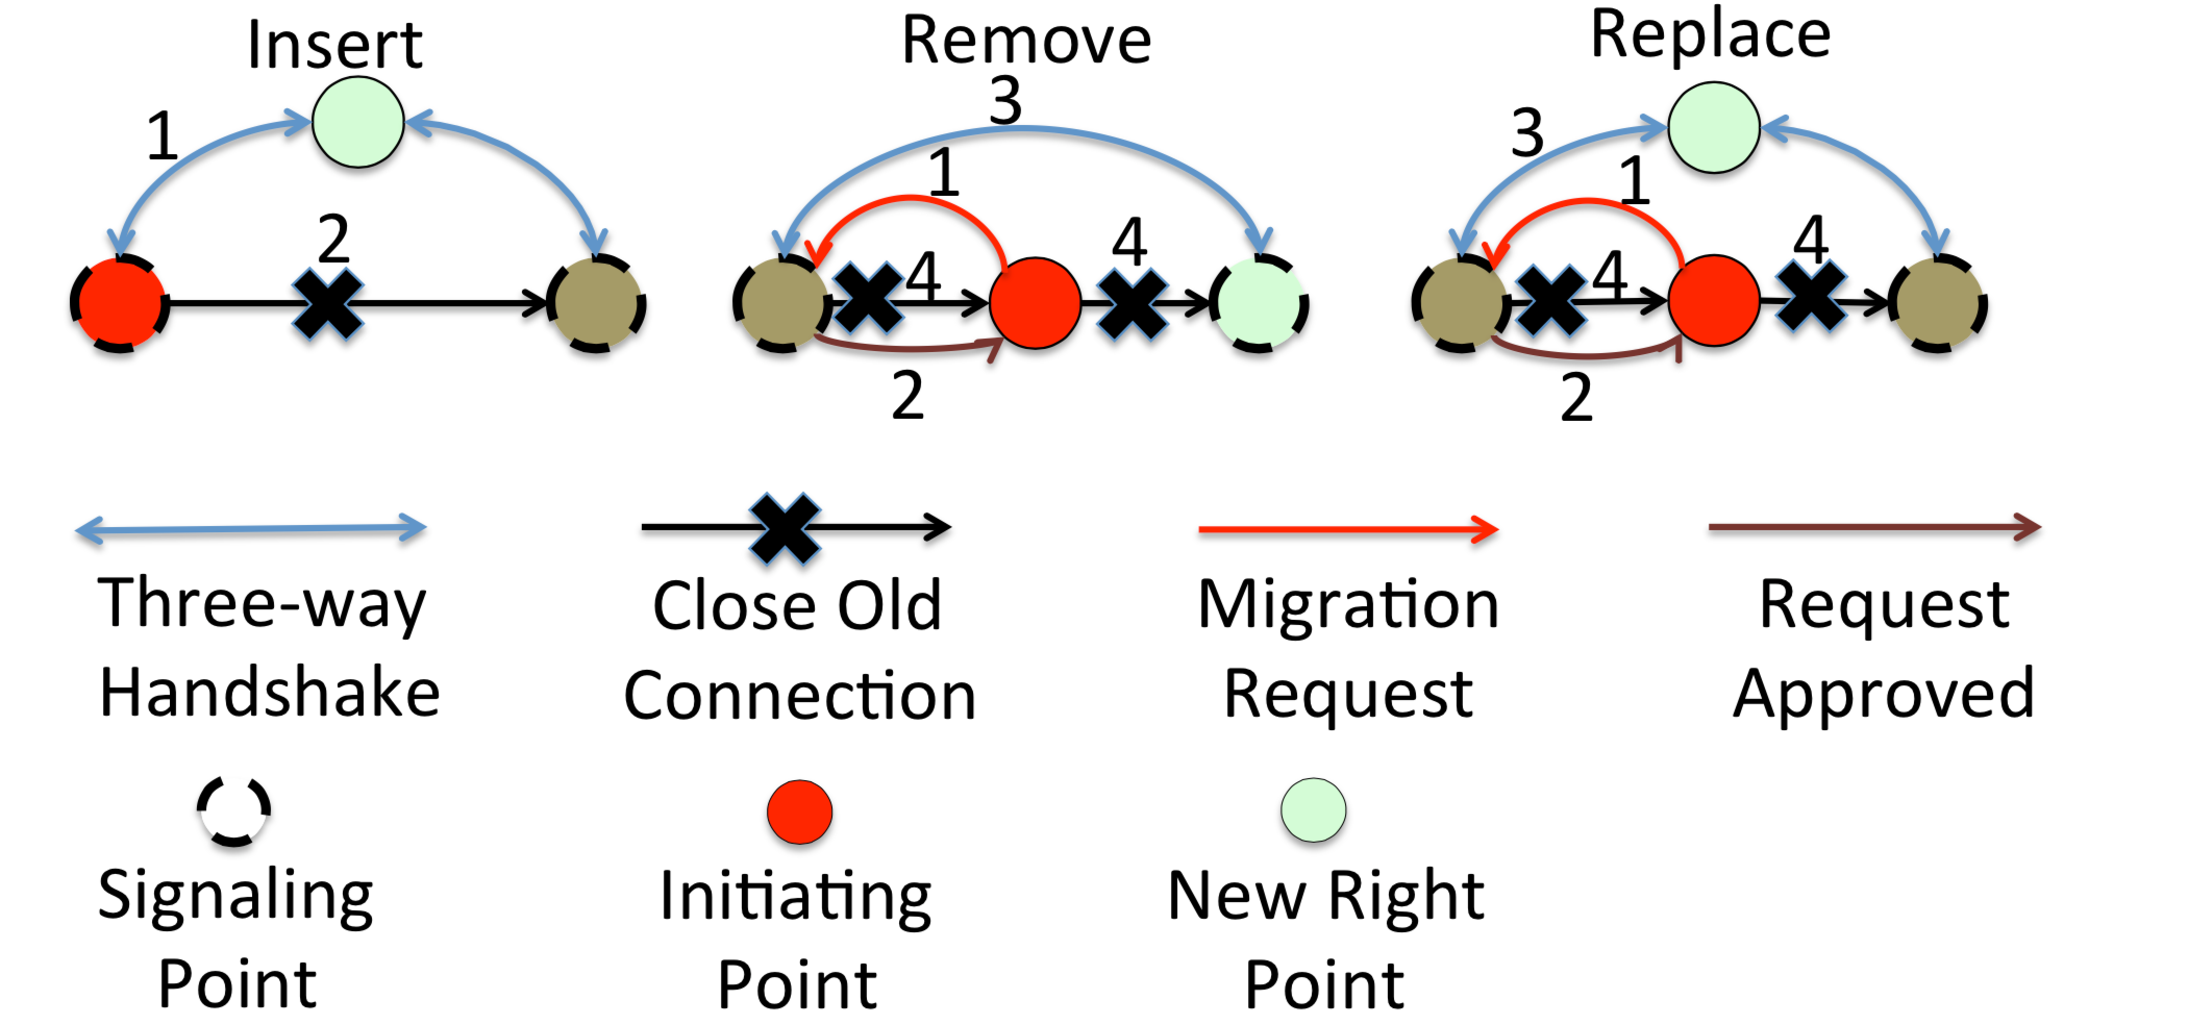
\includegraphics[width=\linewidth]{figures/concurrentupdate.pdf} 
\caption{\small Flow migration during insert, remove and replace}\label{concurfigure}
\end{figure}


\begin{algorithm} [htb]
%\small
\scriptsize

\SetAlgoLined

\SetKwFunction{update}{Trigger\_Migration}\SetKwFunction{IPC}{Msg\_Handler }\SetKwFunction{queue}{Queue Agent}
\SetKwProg{func}{Function}{}{}

\func{\update{} } {
\If{recv(migrate)}
{
  \If{pending == 0} {
  pending++\;
  \If{migration == insert }{
    sendto(New right, UPDATE-SYN)\;
   
  } \Else{
   sendto(Left, request)\;
  }
  }
  \Else{
  Exponentially backoff and retry\;
  }
}


}
\func{ \IPC{} }{
\If{recv(request)}{
  \If{pending$>0$ }{
  sendback(reject)\;
  }
  \Else{
  pending++ \;
  sendto(New right, UPDATE-SYN)\;
  sendback(approve)\;
  }
}

\If{recv(reject) }{
 Exponentially backoff and retry sendto(Left, request)\;
}
\If{recv(approve) }{
//do nothing, to avoid request re-transmission
}

\If{recv(UPDATE-SYN)}
{
  pending++\;
  \If{(migration==insert or replace) and (current == not signaling point) }{
    forward(UPDATE-SYN)\;
  }
  \Else{
  sendback(UPDATE-SYNACK)\;
  } 
  
}
\If{recv(close)}
{
  //clean old flow state\;
  pending$--$\;
}
\If{recv(UPDATE-SYNACK)}{
  pending$--$\;
  \If{(migration==insert or replace) and (current == not signaling point) }{
    forward(UPDATE-SYNACK)\;
  }
  \Else{
  sendto(OldMBox, close)\;
  sendback(UPDATE-ACK)\;
    //clean old flow state\
  } 
  
}
\If{recv(UPDATE-ACK)}{
  pending$--$\;
   \If{(migration==insert or replace) and (current == not signaling point) }{
    forward(UPDATE-ACK)\;
  } \Else{
    //clean old flow state\
  }
 
}

}
\caption{ Concurrent Flow Migration} \label{concurrency}

\end{algorithm} 


\subsubsection{``Break before make''}
\amy{Do you mean ``supersession'' in the following bolded words?}
When a client moves, it may drop the old \textbf{subsession} before establishing a new \textbf{subsession}. Consider when a UE moves across a cell boundary, upon which the UE may suffer from transient connection loss, since it is out of the old cell's range. 

After losing the old \textbf{subsession}, the client needs to rebind to the first hop middlebox. If we use the client's physical IP as part of the supersession identification, the first hop middlebox will fail to identify the supersession if the client changes its IP during mobility. To solve this problem, we can either put the old connection's information in the rebinding message sent by the client or, in a single domain case, administrators can assign a non-routeable IP to each device as a unique ID and use this ID to help identify the supersession. 
 


\section{Data Plane Properties}
In this section, we discuss three data plane properties and the mechanisms that support them atop the control logic. \amy{the data plane is technically below the control logic. Maybe find another word for ``atop''}

\subsection{Loss-Free Update}

%In the migration control logic, we have the concept of ``path''; let us now only focus on data plane and see how path is reflected there.

At the data plane, there is a translation table stored in each middlebox. The \system agent accepts flows for which it has established state, rewrites the header, and forwards the flow based on the supersession-subsession mapping stored in the translation table. Moving a flow from one path to another is equivalent to updating the translation tables at the data plane to accept a flow from the new subsession(s) and reject the same flow from the old subsessions. Since there are multiple middleboxes involved in the update procedure, if the update happens in the wrong order, the translation layer may drop packets, e.g. --- if the old subsession is removed before the new subsession is fully established.


Finding the right sequence of updates for a general network is proven to be NP-complete~\cite{SWAN, zUpdate}, but for a special topology, linear in our setting (we only abstract the topology between middleboxes), we can apply the concept from network consistent update~\cite{consistentupdate, ratul}. We first ensure that all new translation rules are pushed before the egress applies the new rule, and the old rules are not removed until all the new rules are installed via a complete handshake. In particular, when a migration is initialized from the middlebox (a signaling point), the middlebox notifies its neighbor through the control plane, which inserts a new rule for incoming traffic. Then this neighbor notifies the other side of the connection with an UPDATE-SYN control message. Every hop that receives UPDATE-SYN updates its own translation table. Hence once the other signaling endpoint receives the notification, a new rule for the flow has been installed at every hop for one direction of traffic; it is thus safe to apply the new rule for the egress. The opposite direction is set up in the same way with UPDATE-SYNACK messages. Once the new bidirectional path is built, we tear down the old path by removing the old rules. This loss-free update mechanism mirrors the control plane ``make before break'' philosophy and is in fact facilitated by the control plane design. 

 \begin{figure}[ht]
\centering
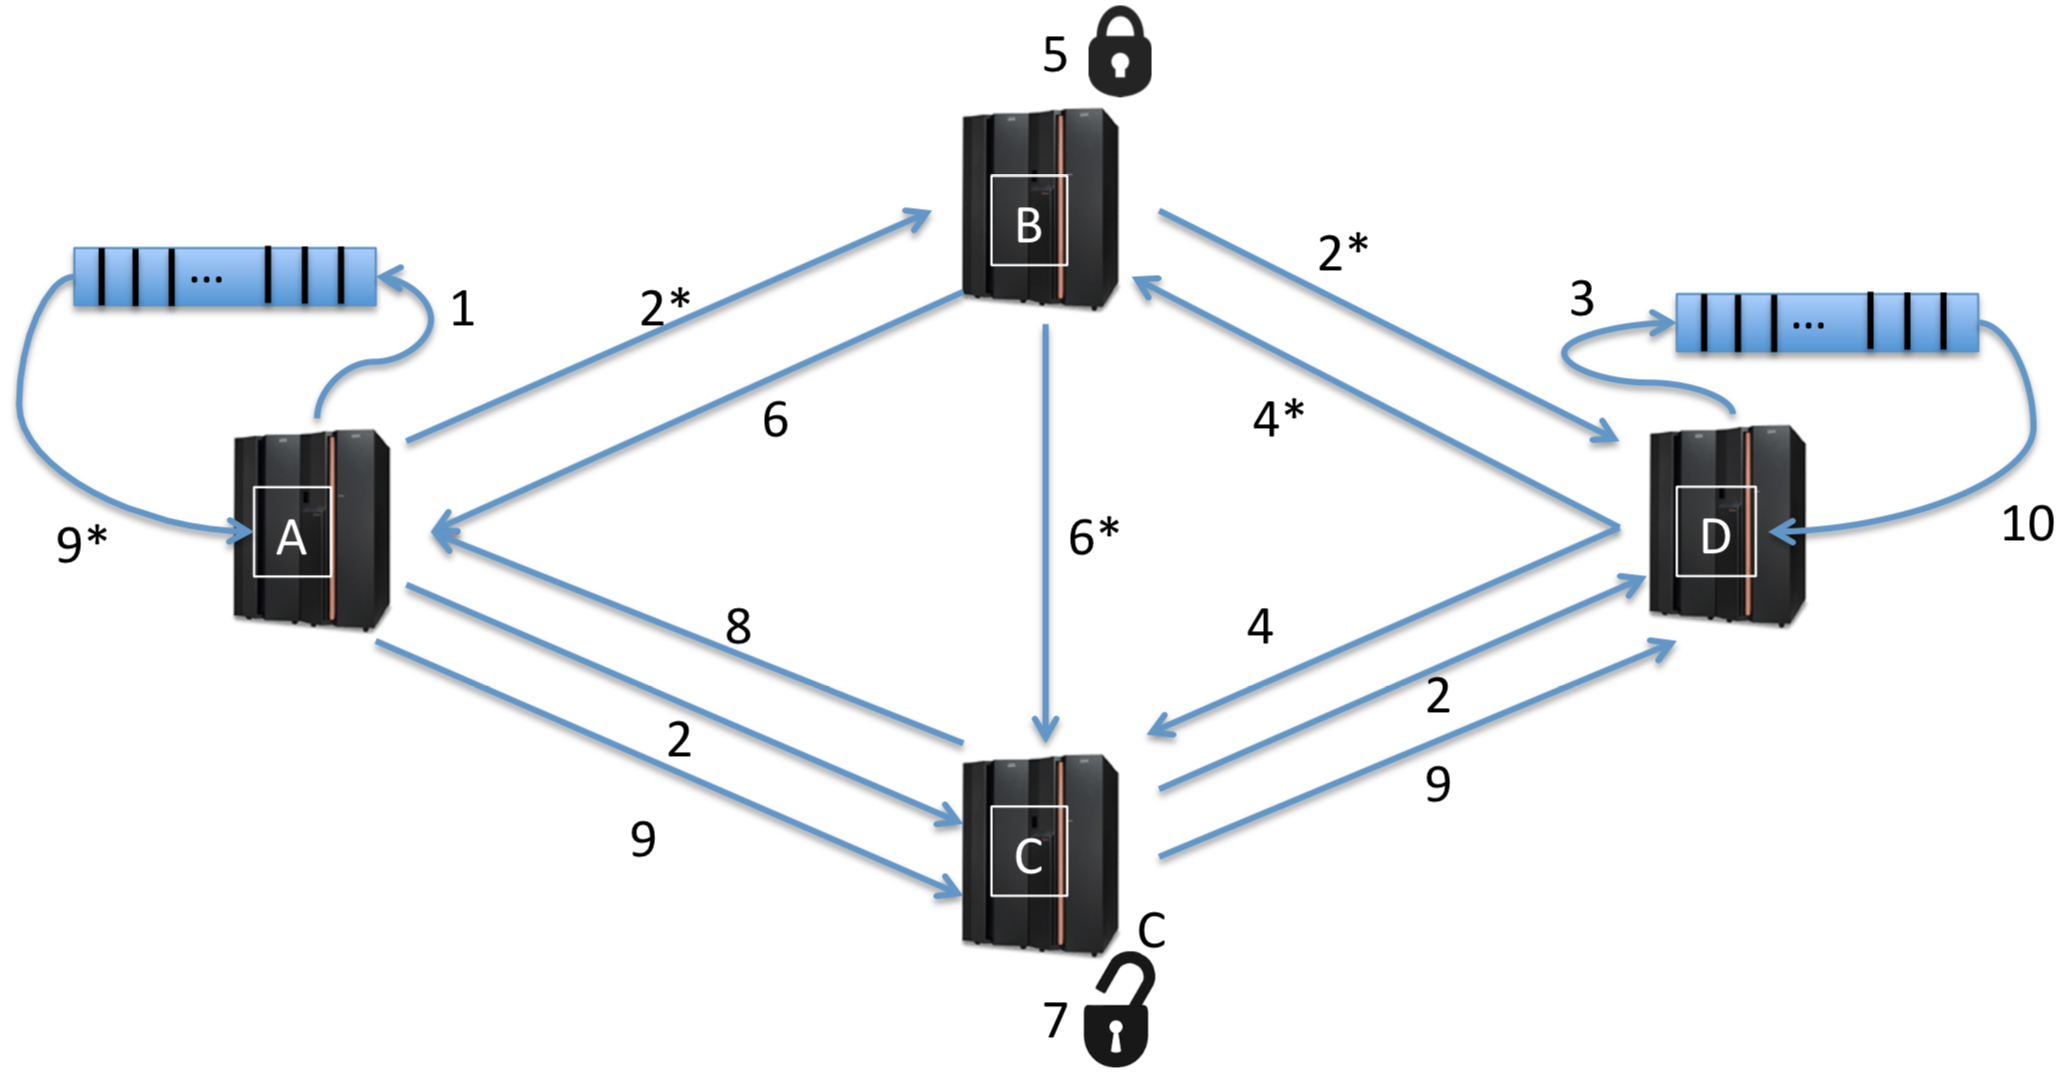
\includegraphics[width=\linewidth]{figures/order_preserving.pdf} 

\caption{Flow Migration in Packet Order Preserving ((a) and (b) can happen in parallel.)} \label{orderpreserving} 
\end{figure}
 
\subsection{Packet Order Preserving} \label{FIFO}
The previously described loss-free update is insufficient if the NF instance (state) also needs to migrate. More specifically, the NF state cannot be migrated since it is being continuously updated as packets are coming in via the old path. To lock and migrate the middlebox state, \system must stop sending traffic during the new path setup. Since changing the protocols' (e.g., TCP) flow control is undesirable, we choose to buffer the traffic and do not release it until the network function state has been replicated at the new path middlebox. Since NF state replication and migration is a well solved problem~\cite{OpenNF, splitmerge, HAMbox}, we do not address this problem here. 

A complete flow and state migration takes 10 steps as depicted in Figure~\ref{orderpreserving}: 
1) lock outgoing traffic; 
2(a) send UPDATE-SYN via new path; 
2(b) send UPDATE-FIN via old path;
3) lock the reverse direction traffic;
4(a) send UPDATE-SYNACK via new path;
4(b) send UPDATE-FINACK via old path;
5) lock middlebox states;
6(a) send UPDATE-FINACK via old path;
6(b) migrate states;
7) unlock middlebox states;
8) send UPDATE-SYNACK via new path;
9(a) send ACK packets;
9(b) release buffered traffic;
10) release buffered traffic for the other direction.
\newline \amy{is this newline intentional}


\begin{figure}[ht]
\centering
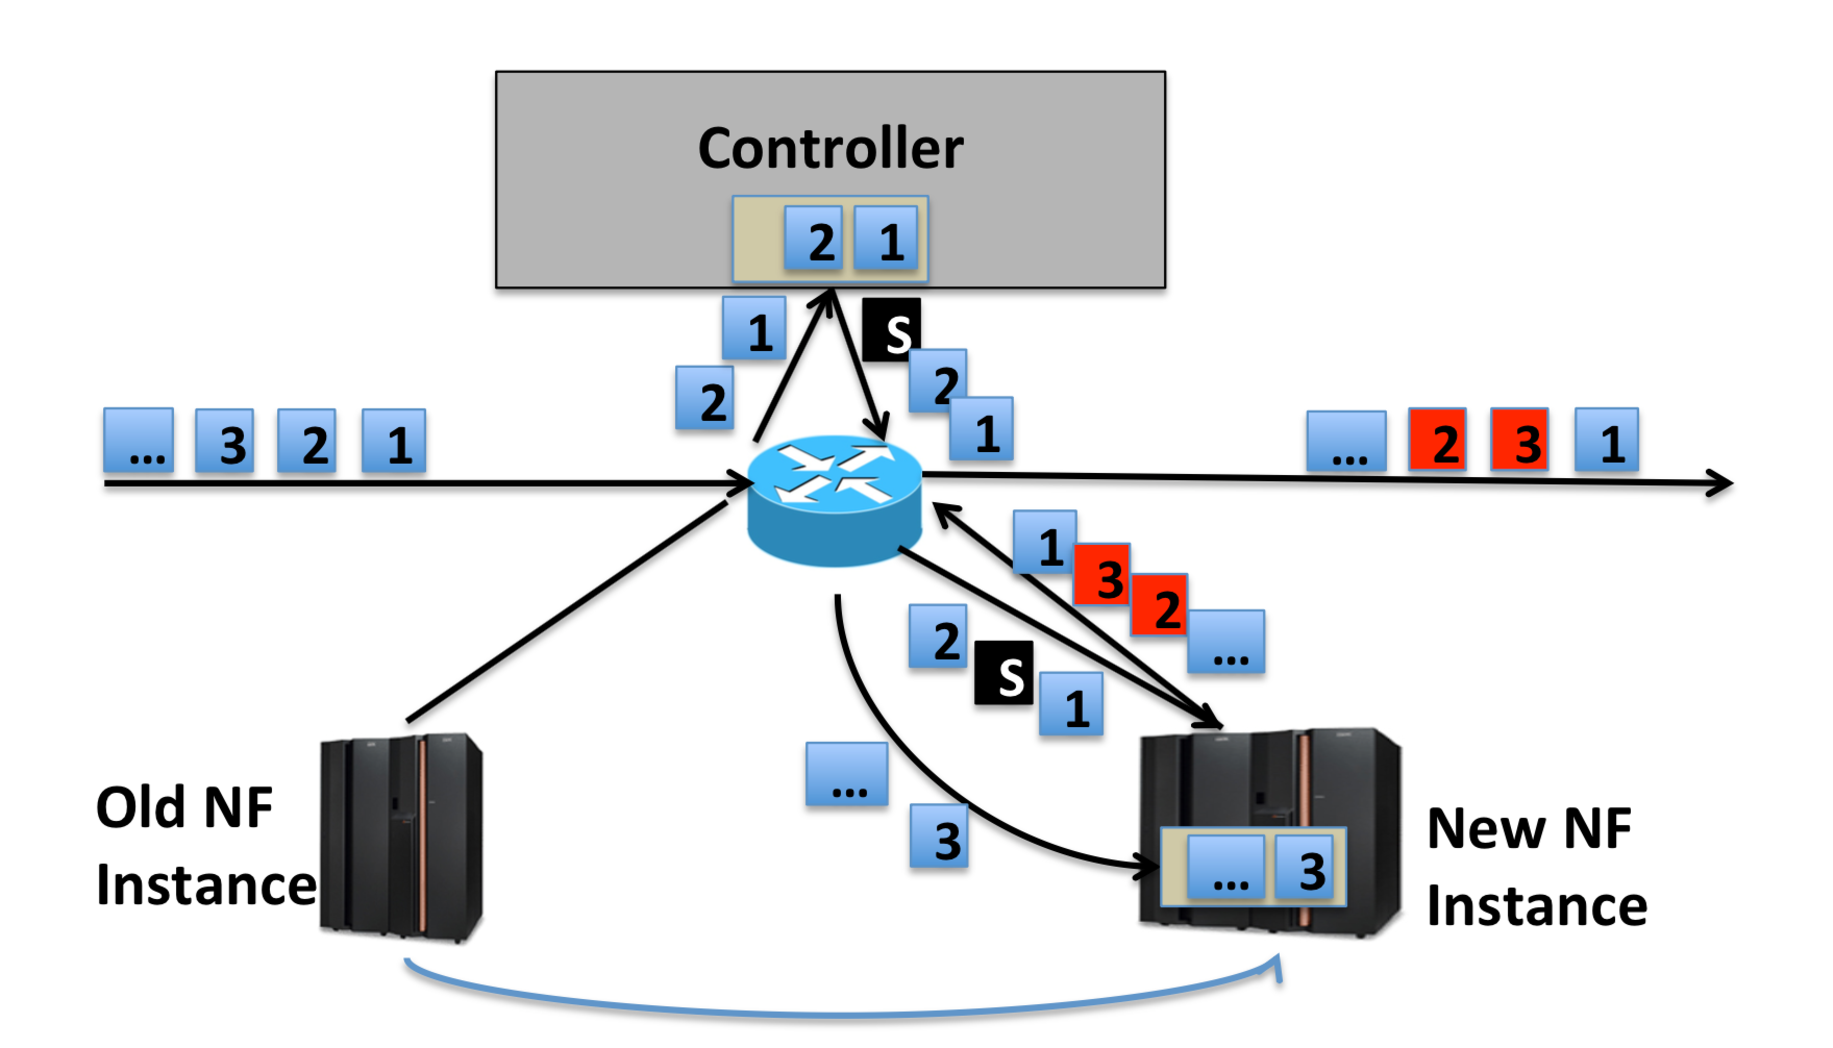
\includegraphics[width=\linewidth]{figures/opennfbroke.pdf} 
\caption{\small Order-preserving problem in OpenNF without FIFO assumption, the signal packet \texttt{s} and the data packets 1 and 2 maybe reordered and thus create reordering. Note the switch is one big switch abstraction.}\label{opennfbroke}
\end{figure}


This update mechanism also satisfies the same \textbf{packet order-preserving} property as defined in OpenNF: assuming the path with the NF instance is \textbf{FIFO}, i.e., the control message sent after the last data packet is always received after the last data packet, \textit{all packets should be processed in the order they were forwarded to the NF instance by the switch (network)}~\cite{OpenNF}. We will now show how we achieve the same property without the FIFO assumption.
 
\subsection{Substream Order Preserving}  

During migration it is useful to create two separate substreams of a byte stream (e.g., TCP), one each for the old and new path. For example, when migrating a flow from one IDS to another, we may want to ensure that all the SYNs and corresponding ACKs go through the same IDS in order to avoid an alert like ``ACK before SYN''. When the flow passes through a deep packet inspection (DPI) NF, both string matching and reg-exp matching build a Deterministic Finite Automaton (DFA), which is traversed from the root based on the byte stream~\cite{aho, yaron}. If we want to use different DPI instances for a byte stream, but the first instance has not seen a complete substream, the first DPI can only check the largest continuous byte stream before it has to buffer the remaining bytes and send them to the second DPI. 


In order to divide substreams cleanly, the left neighbor of the moving node leverages TCP sequence numbers. Suppose a migration is initiated at time $t$. The left neighbor uses the maximum seen TCP sequence number at time $t$ as a \textit{checkpoint}: it buffers packets with a higher sequence number than the checkpoint and forwards packets with a lower sequence number. \system does not lock and migrate the old NF instance state until it sees a TCP ACK with sequence number \textit{checkpoint}. The ACK guarantees the delivery of all the packets in the old substream. Note that although the buffering may create a reordering at the left neighbor middlebox, this protocol results in the correct order for the two substreams from the perspective of endpoints. See Algorithm~\ref{strictorderpres} for details. 


%%%%%%%%%%%%%%%%%%%%%%%%Algorithm %%%%%%%%%%%%%%%%%%%%%%%%%%%%%%%%%%%%%%%%%%%%
%%%%%%%%%%%%%%%%%%%%%%%%%%%%%%%%% %%%%%%%%%%%%%%%%%%%%%%%%%%%%%%%%%%%%%%%%%%%%
%%%%%%%%%%%%%%%%%%%%%%%%%%%%%%%%%  %%%%%%%%%%%%%%%%%%%%%%%%%%%%%%%%%%%%%%%%%%%%
%%%%%%%%%%%%%%%%%%%%%%%%%%%%%%%%%  %%%%%%%%%%%%%%%%%%%%%%%%%%%%%%%%%%%%%%%%%%%%
%%%%%%%%%%%%%%%%%%%%%%%%%%%%%%%%%  %%%%%%%%%%%%%%%%%%%%%%%%%%%%%%%%%%%%%%%%%%%%

\begin{algorithm} [htbp]
\footnotesize
\SetAlgoLined
\SetKwFunction{syn}{recv\_SYN}\SetKwFunction{ack}{recv\_ACK}\SetKwFunction{queue}{release\_queue}
\SetKwProg{mypacket}{Event\_Handler}{}{}
\SetKwProg{func}{Program}{}{}

\mypacket{\syn{TCP\_packet p} } {
checkpoint = hash\_lookup(p)\;
\If{p.seq $>$ checkpoint} {
Buffer (p)\;
} 
\Else{Forward(p)\;}
} 


\mypacket{\ack{TCP\_packet p}}{
\If{p.ack $>$checkpoint}{
Migrate NF state\;
//wait until migration finishes\;
sendto(left neighbor, release\_buffer)\;
}
}


\mypacket{\queue{}}{
\While{!buffer.empty()}{
Forward(buffer.dequeue())\;
}
Reset(hash\_table)\;
}

\caption{Substream Order Preserving} \label{strictorderpres}
\end{algorithm} 


%%%%%%%%%%%%%%%%%%%%%%%%Algorithm %%%%%%%%%%%%%%%%%%%%%%%%%%%%%%%%%%%%%%%%%%%%
%%%%%%%%%%%%%%%%%%%%%%%%%%%%%%%%% %%%%%%%%%%%%%%%%%%%%%%%%%%%%%%%%%%%%%%%%%%%%
%%%%%%%%%%%%%%%%%%%%%%%%%%%%%%%%%  %%%%%%%%%%%%%%%%%%%%%%%%%%%%%%%%%%%%%%%%%%%%
%%%%%%%%%%%%%%%%%%%%%%%%%%%%%%%%%  %%%%%%%%%%%%%%%%%%%%%%%%%%%%%%%%%%%%%%%%%%%%
%%%%%%%%%%%%%%%%%%%%%%%%%%%%%%%%%  %%%%%%%%%%%%%%%%%%%%%%%%%%%%%%%%%%%%%%%%%%%%


A combination of order preserving and substream separation provides us with a stronger \textbf{substream order preserving} property during an update: \textit{substreams should be processed by different NF instances in the order they were sent from the sender}. OpenNF cannot guarantee order preserving with respect to a byte stream when network links are not FIFO~\footnote{OpenNF tech report relies on this assumption in its proof.}. Furthermore, because OpenNF is by design router-based, it simply \textit{cannot} achieve substream order preserving; see Figure~\ref{opennfbroke}. Our protocol is able to provide this property precisely because the system architecture is designed to be aware of and rely on transport protocols.


Note that we may need to split the packets in the case of SYN-ACK piggyback and packet coalescing. In the first case, both directions asking for substream separation can result in deadlock since \system may choose the new path for a substream with higher sequence number in one direction and the old path for ACK as it is ACK-ing a substream with lower sequence number in the reverse direction. In the second case, the TCP client may coalesce packets, causing the payload  to cross the \textit{checkpoint} boundary in the byte stream if retransmission occurs. 








\section {Implementation}

\subsection{Prototype}

There are    three  options   for  an in-kernel
implementation of the data plane: (i) OS  native  network stack; (ii) NIC
driver (e.g.,  DPDK~\cite{dpdk});   and  (iii)   customized  in-kernel
software switch (e.g.,  openvswitch~\cite{ovs}).  We chose option (i) because (a) \system has  to choose the  right interface before sending to
the driver   when  having  multiple  interfaces;  and  (b)  a customized
in-kernel software switch has high overhead.  We implement  a kernel module data  plane  and user  space control/management
plane via TCP/UDP sockets, with a total of about 4000 lines of code in
C  and   C++.   We install kernel modules to
register callback  functions with  Linux  \texttt{netfilter}  for data
plane operations. The   control/management  plane  has    extensible,
complex control logic, and the data plane does specific, simpler actions
such as header rewriting, queuing packets to user  space via \texttt{netfilter\_queue} and  updating the
kernel hash table, which holds the flow $\rightarrow$ port mapping.  The user and the kernel  agent  communicate via 
\texttt{netlink}, a native   Linux  Inter Process Communication  (IPC)
function.  Currently the policy server  is   a simple TCP server  that
proactively pushes policies to the agents.

\begin{figure}[ht]
\centering
% 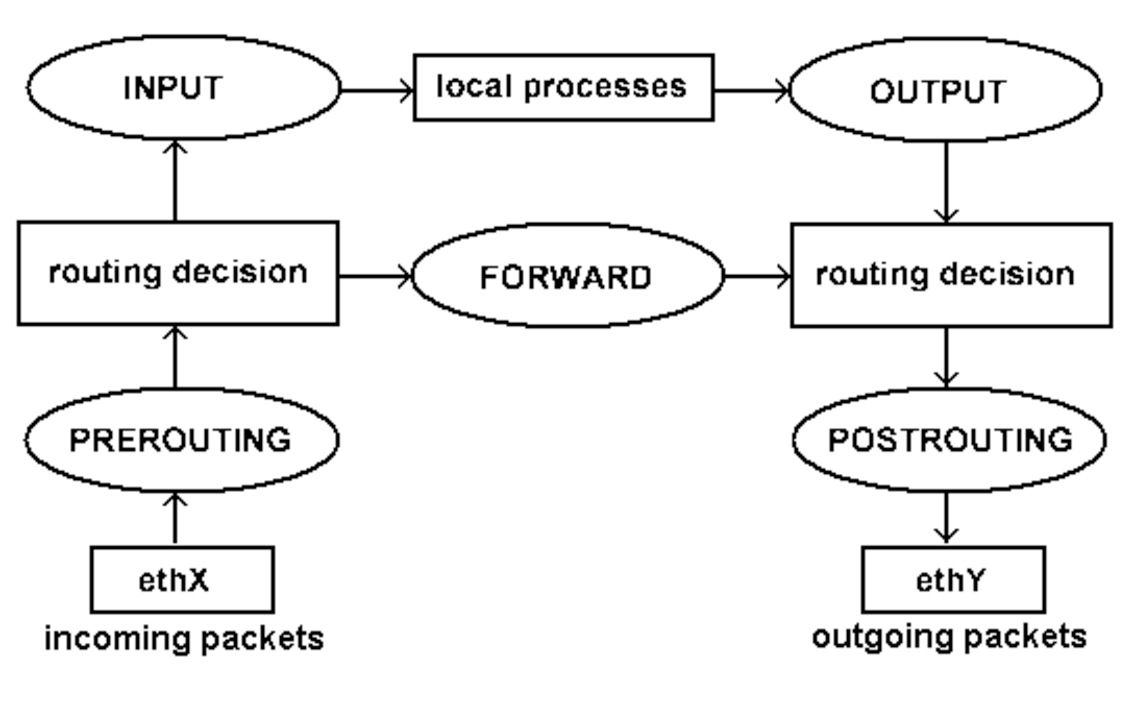
\includegraphics[scale=0.25]{figures/netfilter.pdf} 
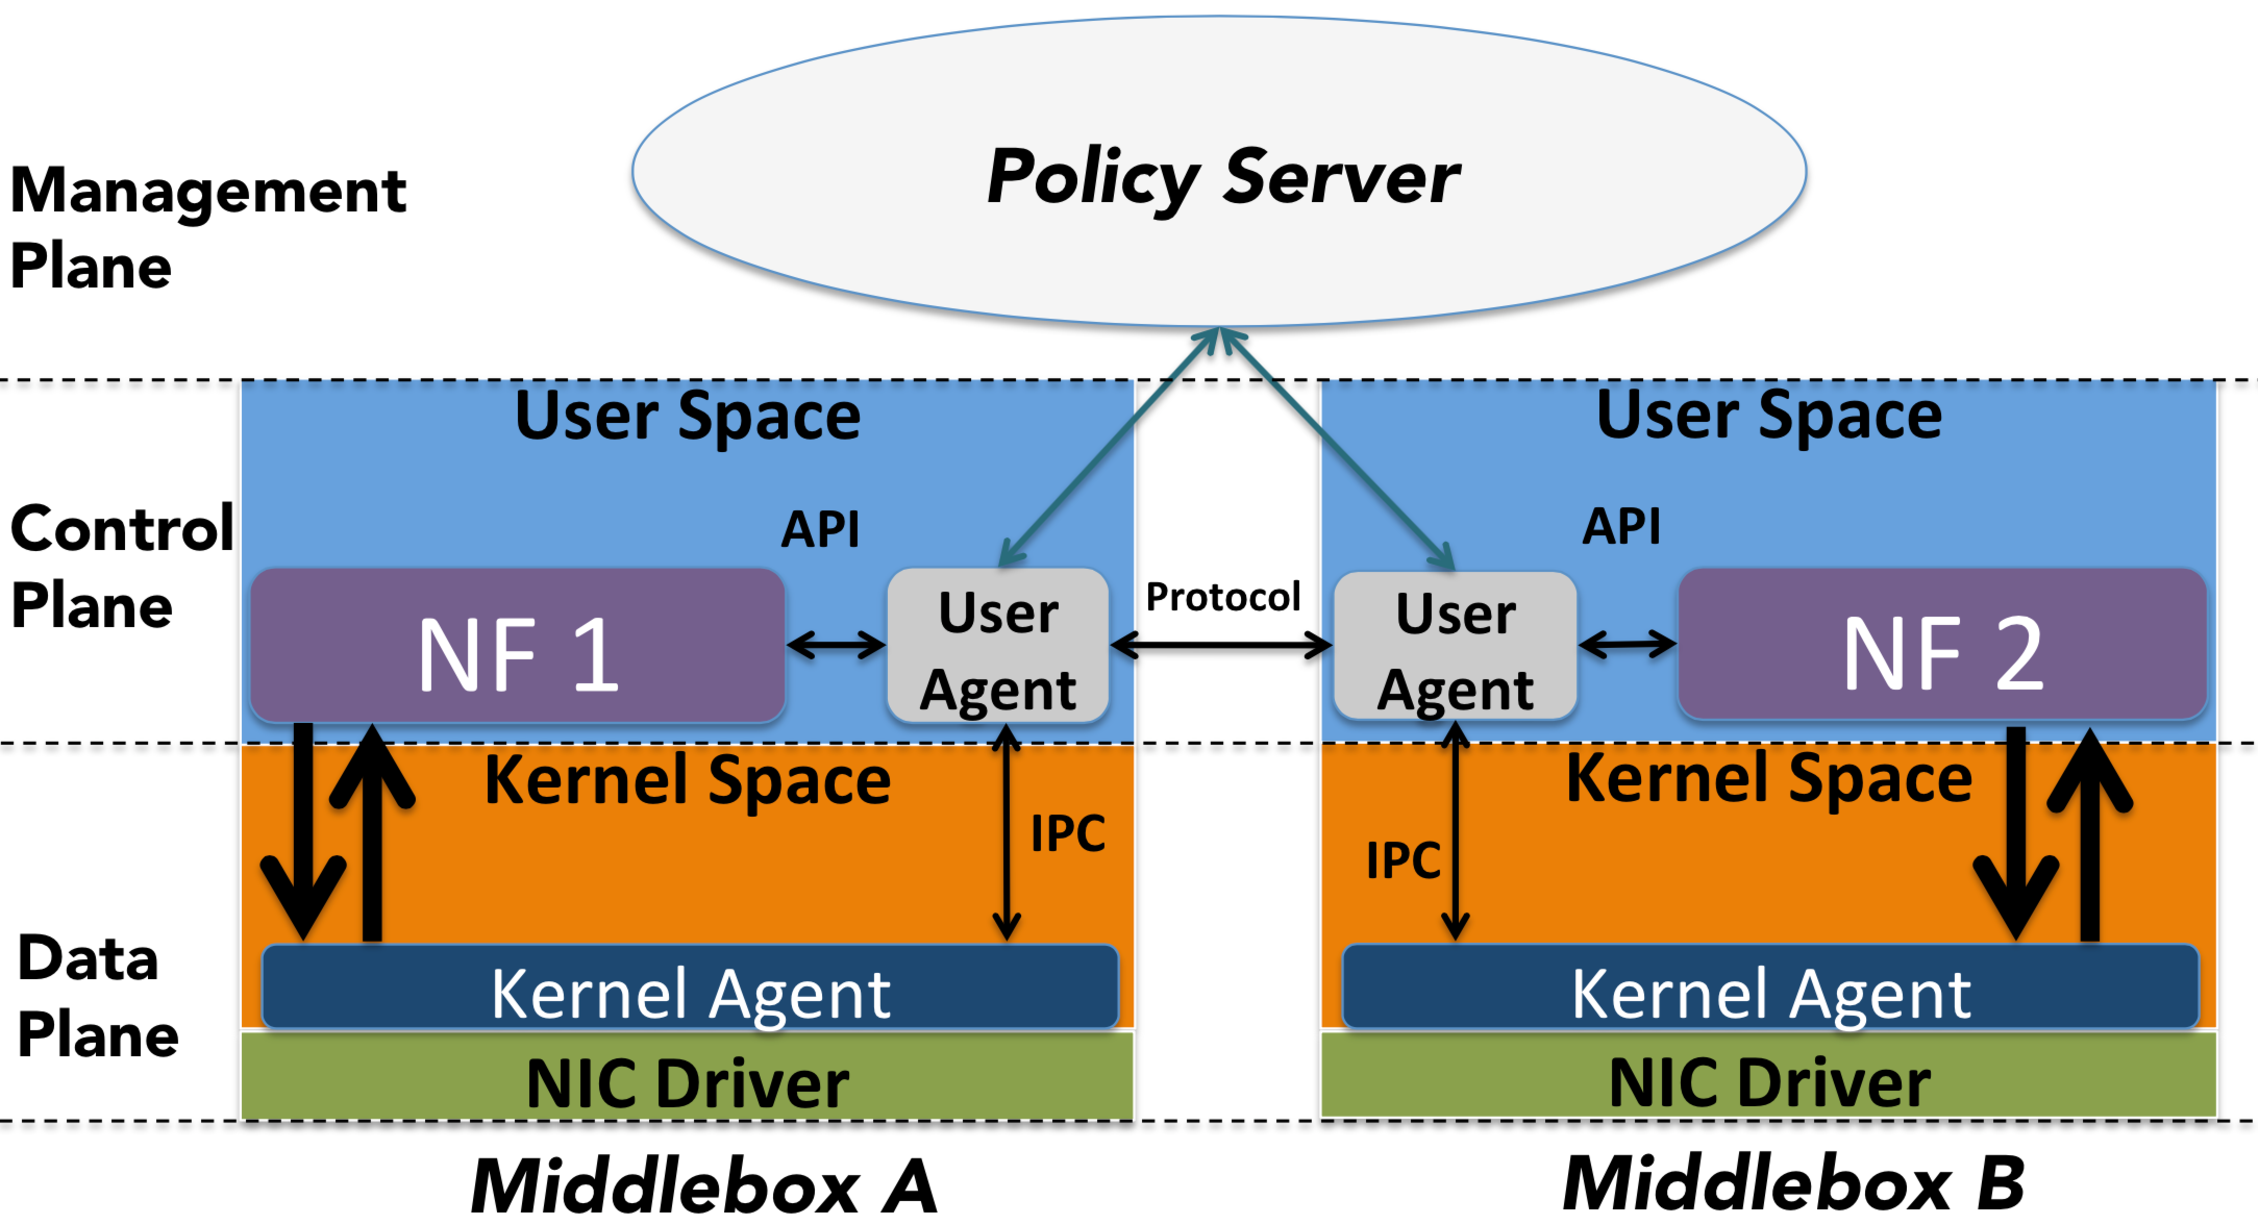
\includegraphics[width=\linewidth]{figures/archiIllustrrate.pdf} 

\caption{\small Layout of the implementation blocks}\label{netf}
\end{figure}





\subsection{Network Function Support}\label{sec:NFsupport}

We categorize NFs into two types --- active and passive functions --- based on whether the NF acts on the original packet.  

\begin{table}[ht]\label{middleboxextension} 
\centering
 
\small
\begin{tabular} {|l |c |c |c|}
\hline

      Name          	  &         Type           & Key        	 &      Binding   \\
                      	  &                        &  Functions          &       Library  \\ \hline
PRADS~\cite{prads} (P) 	  &      Monitoring        &    got\_packet()      & libpcap   \\ \hline
Bro~\cite{bro} (P)      	  &      IDS               &   DumpPacket()      & libpcap   \\ \hline
Snort~\cite{snort} (P)  	  &        IDS         &    PQ\_Show()          & libpcap \\ \hline 
Balance~\cite{balance} (A)	  &      Load Balancer     &    recv(), writen()       &user socket\\ \hline
Squid~\cite{squid} (A) 	  &        Proxy           &  getsockopt()        & user socket  \\ \hline
Traffic- 		  &    WAN-                &     net\_receive       &Linux  \\ 
Squeezer~\cite{tsqueezer} (A)&Optimizer &\_skb()   & skbuff \\ \hline


\end{tabular}
\caption{\small Commonly-used Network Functions; (A) means active and (P) means passive NF. }\label{nfhook}
\end{table}


 Many passive NFs make decisions based on a clone of the original packet. Based on our survey in Table~\ref{nfhook}, we found that most passive NFs use libpcap to capture cloned packets from a raw socket. As described in \S\ref{sec:arch}, we must restore the supersession header of the copies before delivering them to the NF. 
To implement this so-called vertical NAT, we modified the \texttt{pcap\_handle\_packet\_mmap()} function in \texttt{pcap-linux.c} in libpcap~\cite{tcpdump} to restore the supersession. 

For active NFs, there are two cases. If the NFs only act on the payload or MAC layer, e.g.--- TrafficSqueezer, supersession restoring also works. 
However, if the NF acts on the 5-tuple, we have to extend NF functions to notify the \system agent of its header mapping. 
For example, a transparent cache proxy~\cite{squid} gets the packets from its listening port and sets up a new TCP socket to the final destination. \system will break the supersession into two if it is unaware of the mapping between two sessions. On the other hand, if the NF informs the \system agent of the mapping between its listening and sending TCP sockets, the \system agent can stitch the two subsessions into the same supersession. 
 



% \subsection{Middlebox Support}




% 
%Three way handshake
%read write lock
%kmalloc atomic for faster access


\section {Evaluation}


In our evaluation, we demonstrate that:

\begin{itemize}
 \item The system can sustain very high throughput
 \item The system has extremely low latency for flow migrations
 \item The system is resilient to lossy network and update failure. 
\end{itemize}


The testbed we used for evaluation consists of two sets of machines: (i) four mid-range workstations (Quad-core Intel Xeon 3.7GHz, 32GB, 1Gbps NIC) and a conventional switch; and (ii) four high-end servers (16-core Intel Xeon 2.2GHz, 64GB, 40Gbps NIC) with an OpenFlow-enabled switch (we only use L-2 switching here). We conducted throughput stress tests in the four high-end servers, and unless specified, experiments are done in setting (i). 



\subsection{Throughput }

We show that an in-kernel implementation of the shim layer has very low overhead in the overall system. 


\begin{figure}[ht]
\centering
% 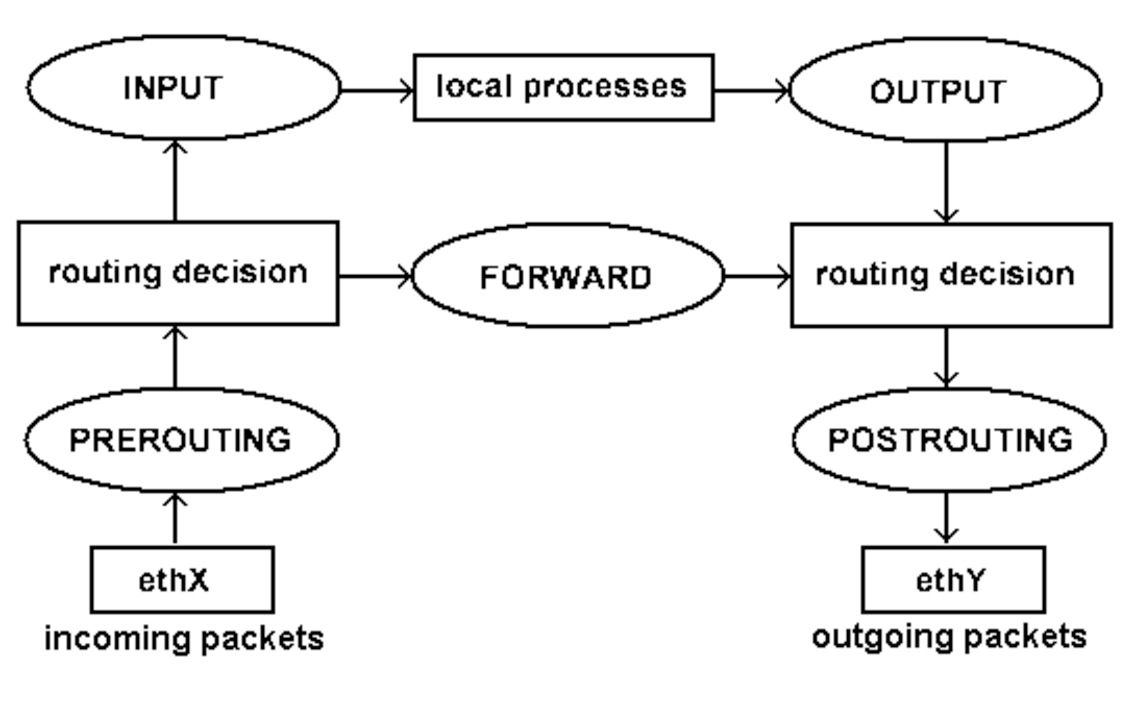
\includegraphics[scale=0.25]{figures/netfilter.pdf} 
% 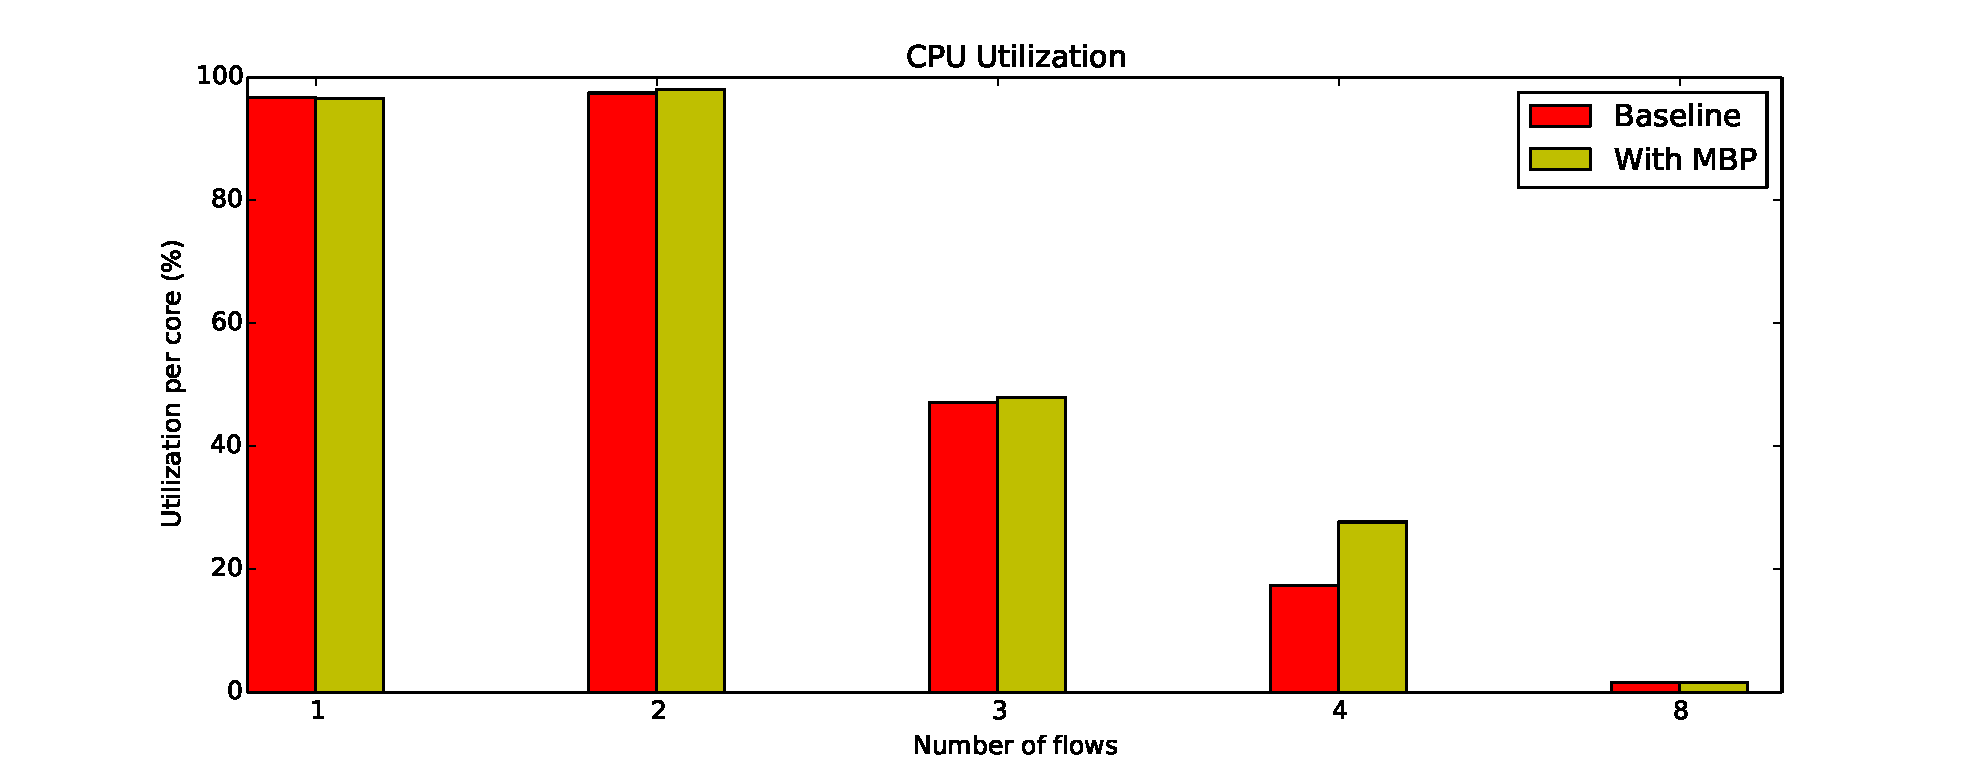
\includegraphics[width=0.53\linewidth]{figures/CPU.pdf} 
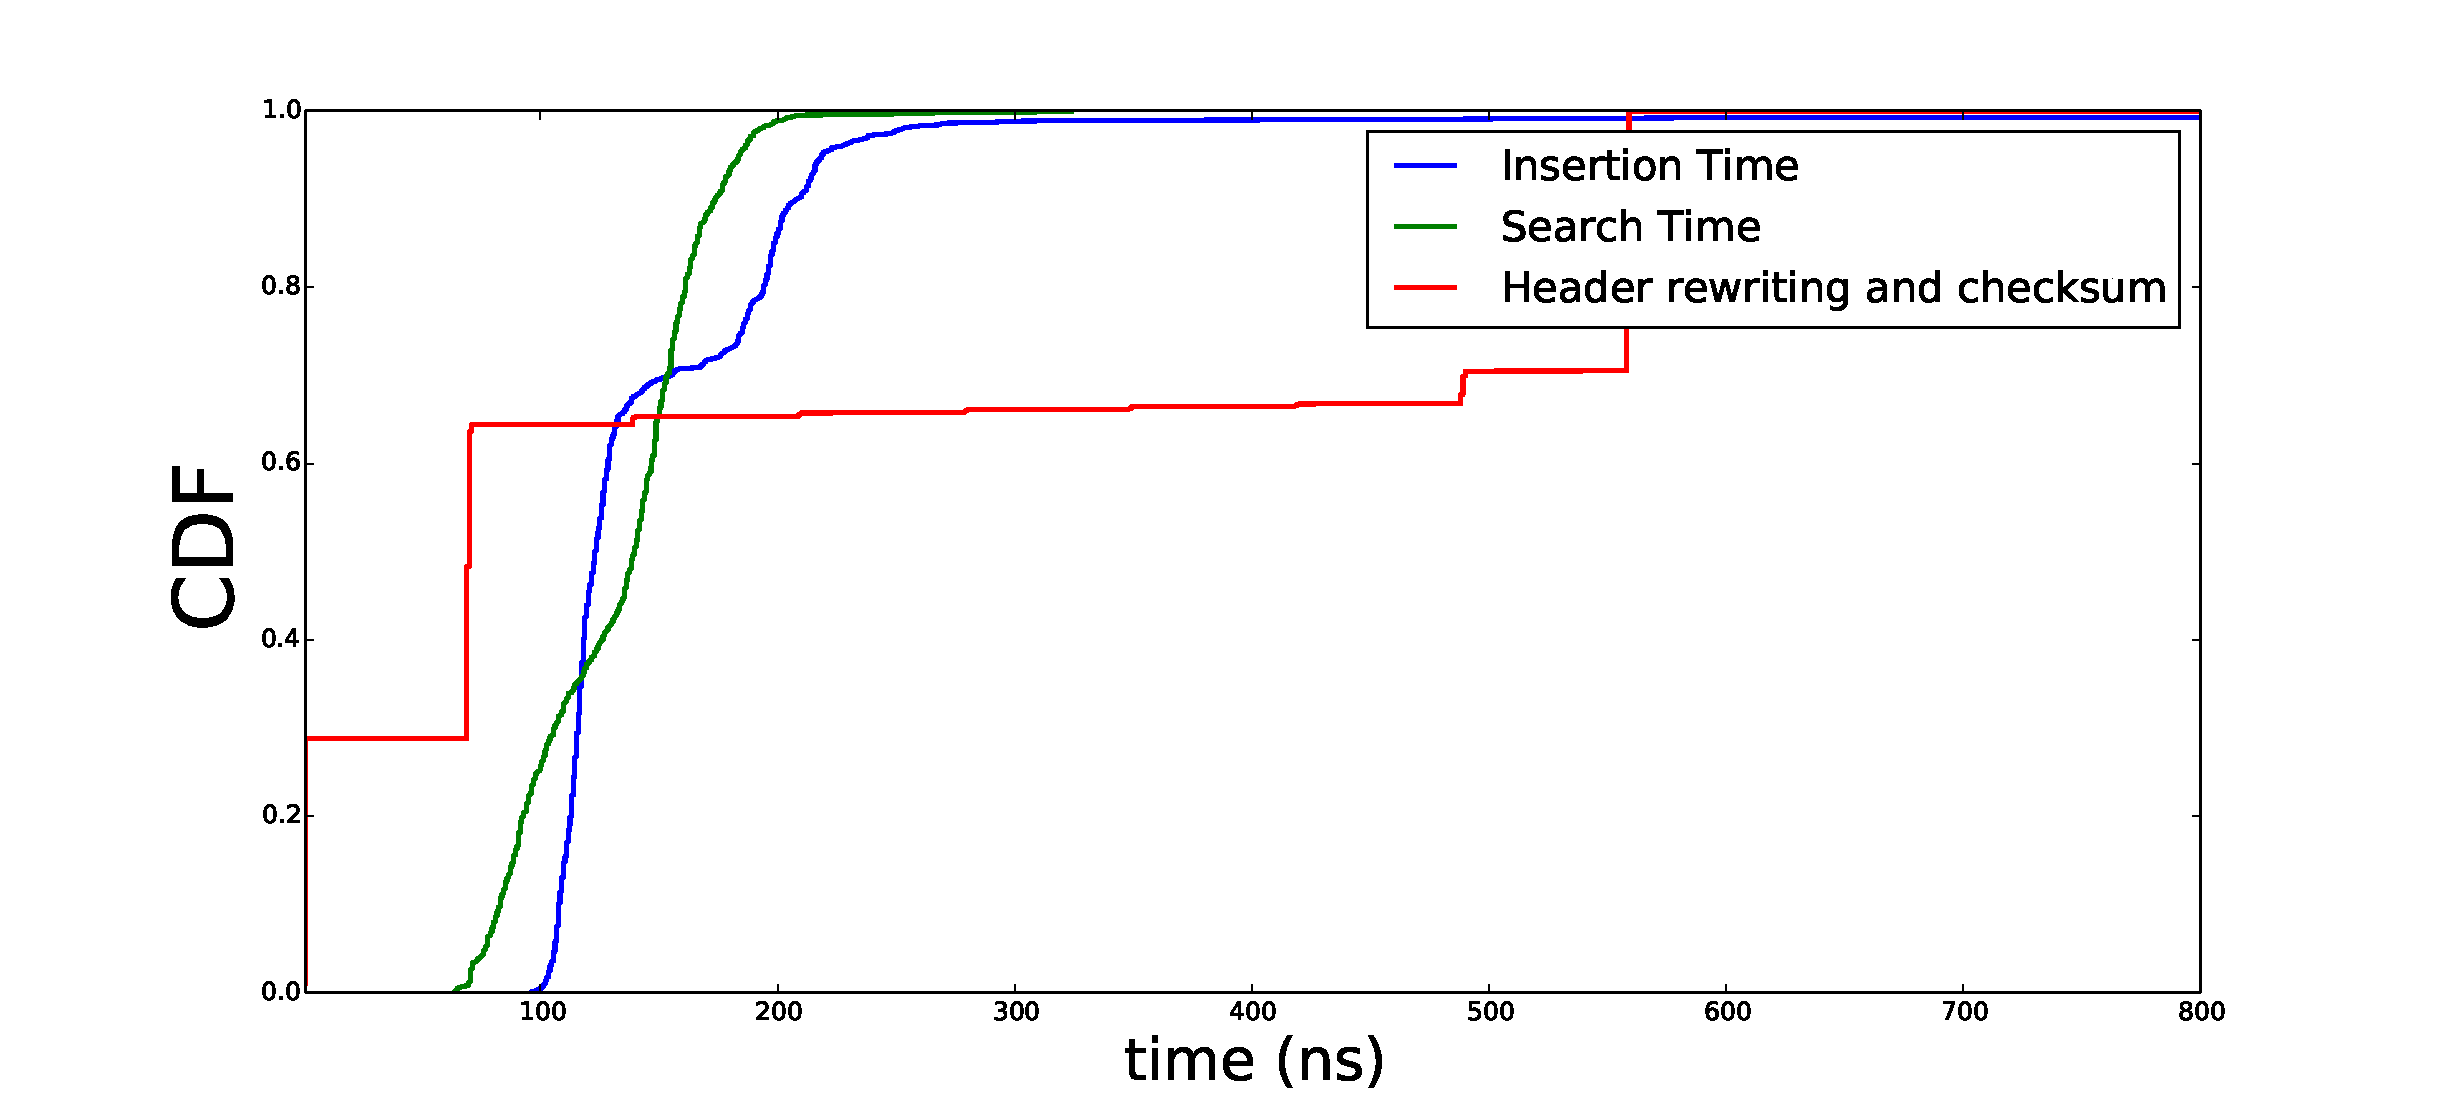
\includegraphics[width=\linewidth]{figures/cdf.pdf} 
\caption{\small Time CDF for different functions}\label{throughput}
\end{figure}
% 

The in-kernel implementation of the data plane includes three functions: (i) action hash lookup, (ii) header rewriting and re-checksum, (iii) rule installation. We also have a few optimizations in the data-plane implementation (e.g., partial checksum to reduce CPU cycle, a small hash table to fit in L3 cache) result in an extremely efficient system with a very low overhead.

We conducted a microbenchmark to see the delay different functions add to the system. We insert 100K rules in the kernel hash table, and conducted 100K lookup. We also microbenchmarked the header rewriting and partial checksum of the data packets. We had the two following methods to eliminate Linux timer's overhead: (i) batch and time the insertion and lookup for every one hundred rules; (ii) get the pure timer lookup time and then subtract that base number. The result shows that lookup, insertion and header rewriting takes on average 131, 251, and 214 ns, this gives us $\approx $ 2.8M packets per seconds with lookup and header rewriting, this is equivalent to 33.6 Gbps per core with MTU of 1500 Bytes.



\begin{figure}[ht]

\centering
% 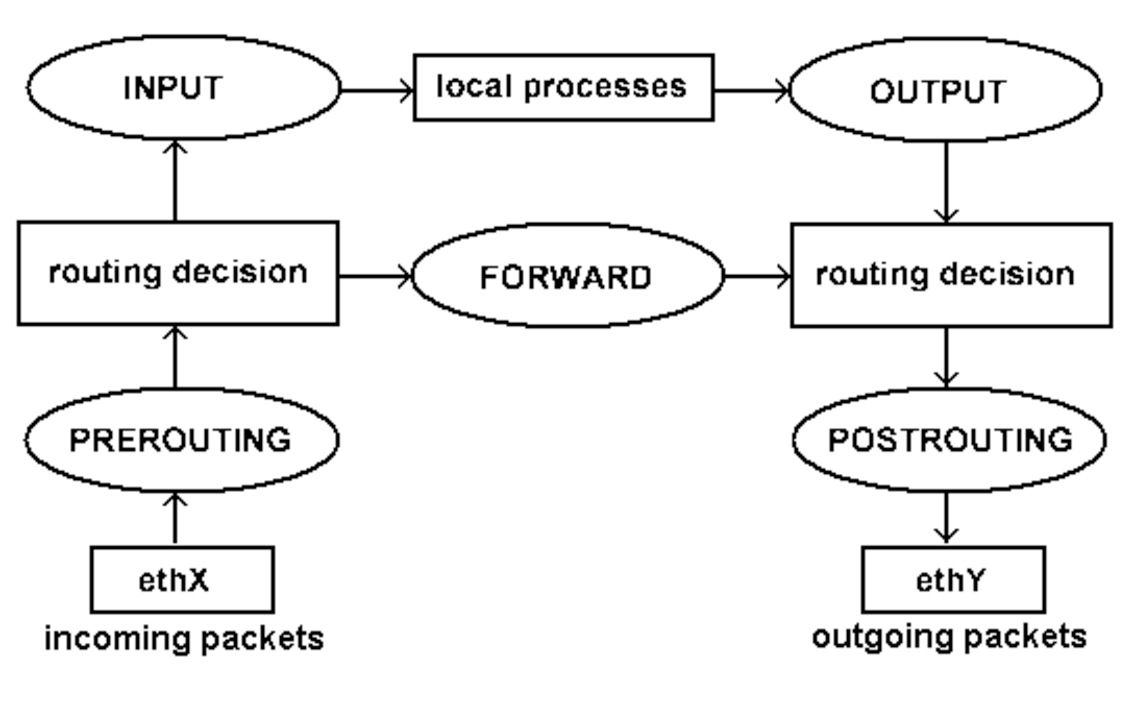
\includegraphics[scale=0.25]{figures/netfilter.pdf} 
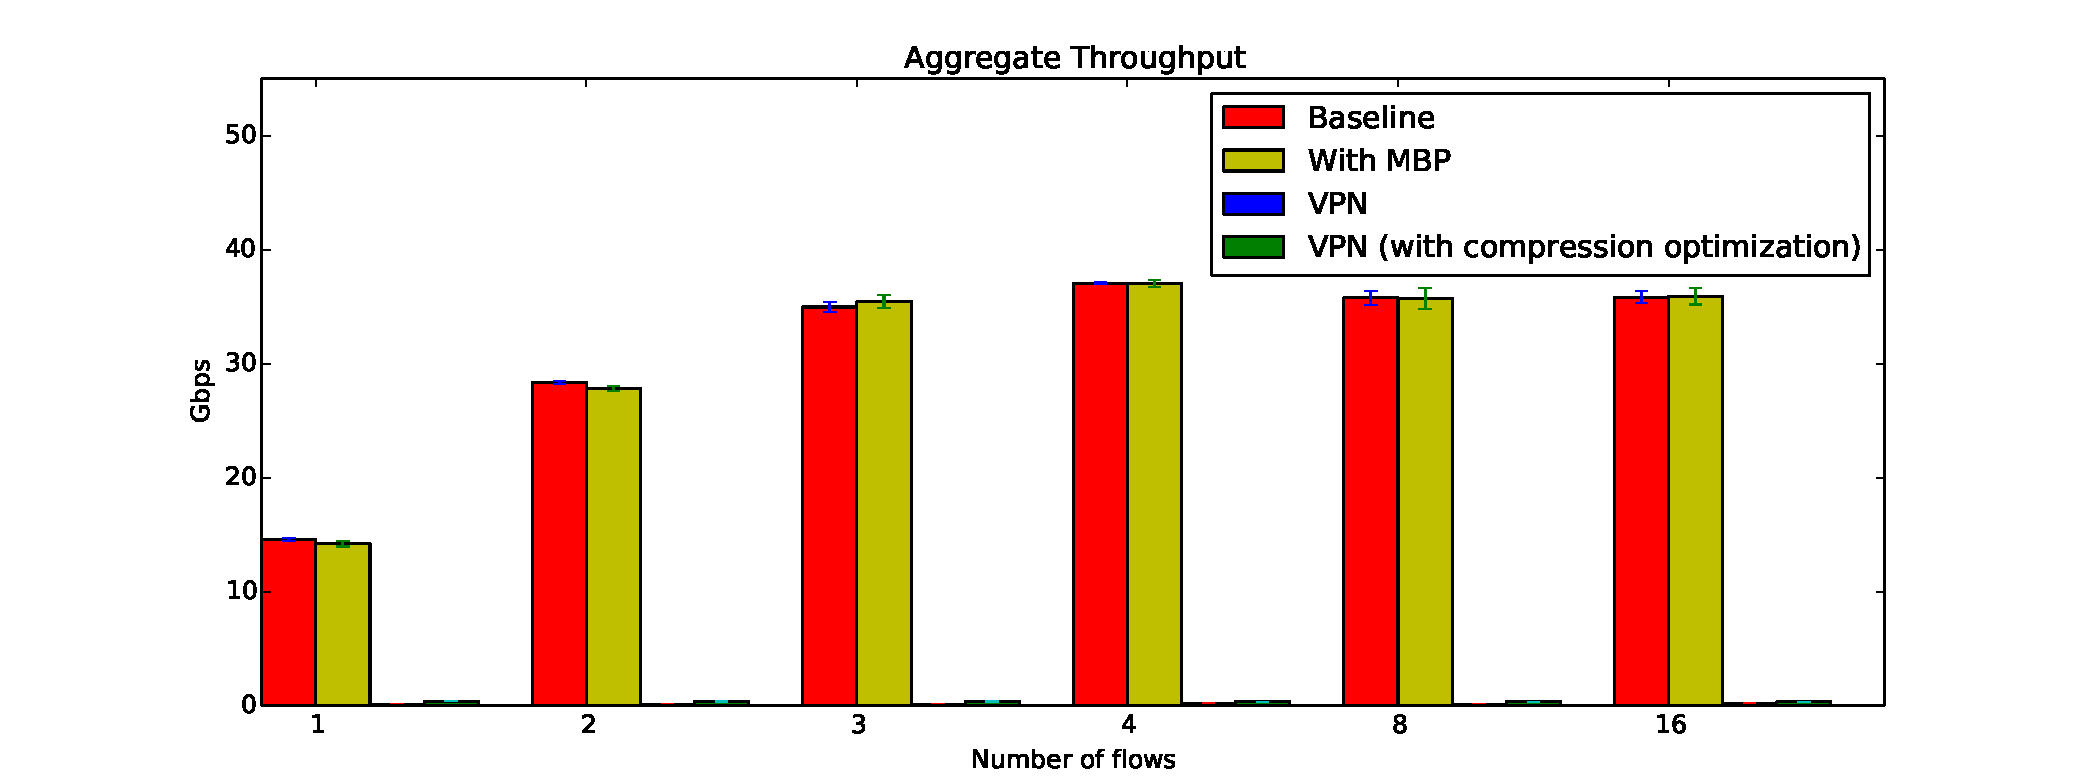
\includegraphics[width=\linewidth]{figures/throughput.pdf} 

\caption{\small Throughput of different approaches. The throughputs are averaged over 20 samples and the error bars show 95\% confidence intervals. Note each flow is hashed to one queue and thus binded to one core during CPU interrupts.}\label{throughput} 
\end{figure}

To test the throughput, we run iperf~\cite{iperf} with MTU of 1500 Bytes on three high-end machines with one \textbf{40 Gbps} port. The topology is client-to-middlebox-to-server, and we use a simple three-hop routing as baseline. We also changed the NIC's ring buffer hash function to an XOR hash function to avoid core interrupt collision, since the default hash function is designed for large number of flows, we see noticeable collision, i.e., hash two flows to the same ring buffer when the number is small.

The in-kernel data plane implementation can sustain \textbf{14.2 Gbps} for a single core, and scale near-linearly to the number of cores, and reaches \textbf{37.1 Gbps} at its peak. (The gap between this and 40 Gbps is due to the way how the bandwidth is calculated, this only computes payload $\leq$ 1460 Bytes versus ethernet frame 1518 Bytes).

To put in perspective, the baseline without running our kernel module can support \textbf{14.6 Gbps}, so the kernel module's overhead is under \textbf{3\%}. The gap is closing as we increase the number of flows, since it incurs less frequent interrupts per core (the frequency of per-core interrupt for 4 flows with 9 Gbps per flow is 66\% of a single flow with 14.5 Gbps), and thus the stress per core is lighter. We envision if we increase the NIC bandwidth to 100 Gbps or higher, the gap will stay the same and the throughput will grow near-linearly before the PCI becomes the bottleneck. 

One interesting observation is that when there are three flows, the system offers a higher throughput than the baseline. The reason behind it is that the ``extra work'' tends to keep the cores busy and thus gets more CPU cycles for processing. The competing flows from TCP congestion control may also affect the throughput. 

We compare our approach with off-the-shelf VPN-encapsulation mechanism, which is used in APLOMB~\cite{Aplomb} system to achieve its redirection. Not surprisingly, VPN uses encryption and thus offers much lower throughput. OpenVPN~\cite{openvpn}, which is used in APLOMB system can only achieve $<$\textbf{400 Mbps} for a single thread, even with the compression optimization. Current OpenVPN does not support multi-threading, even if OpenVPN supports multi-threading in the future and assume it scales linearly to 16 cores, it can only offer 17\% of the max throughput. 

\begin{figure}[ht]
\centering
% 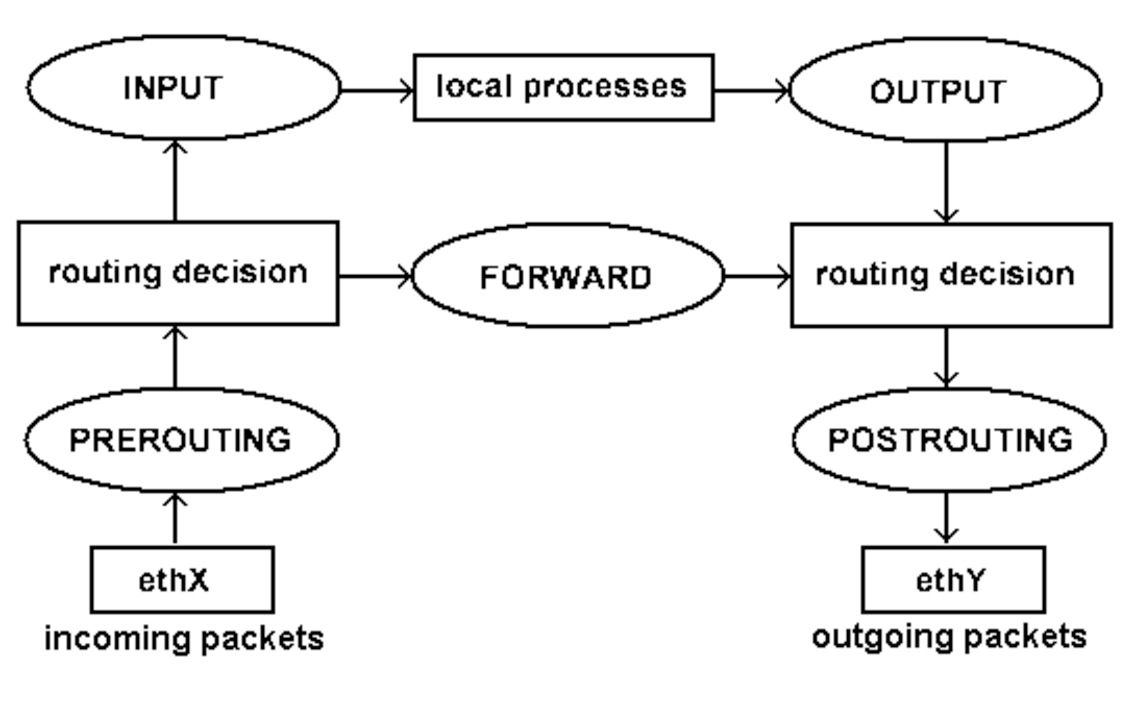
\includegraphics[scale=0.25]{figures/netfilter.pdf} 
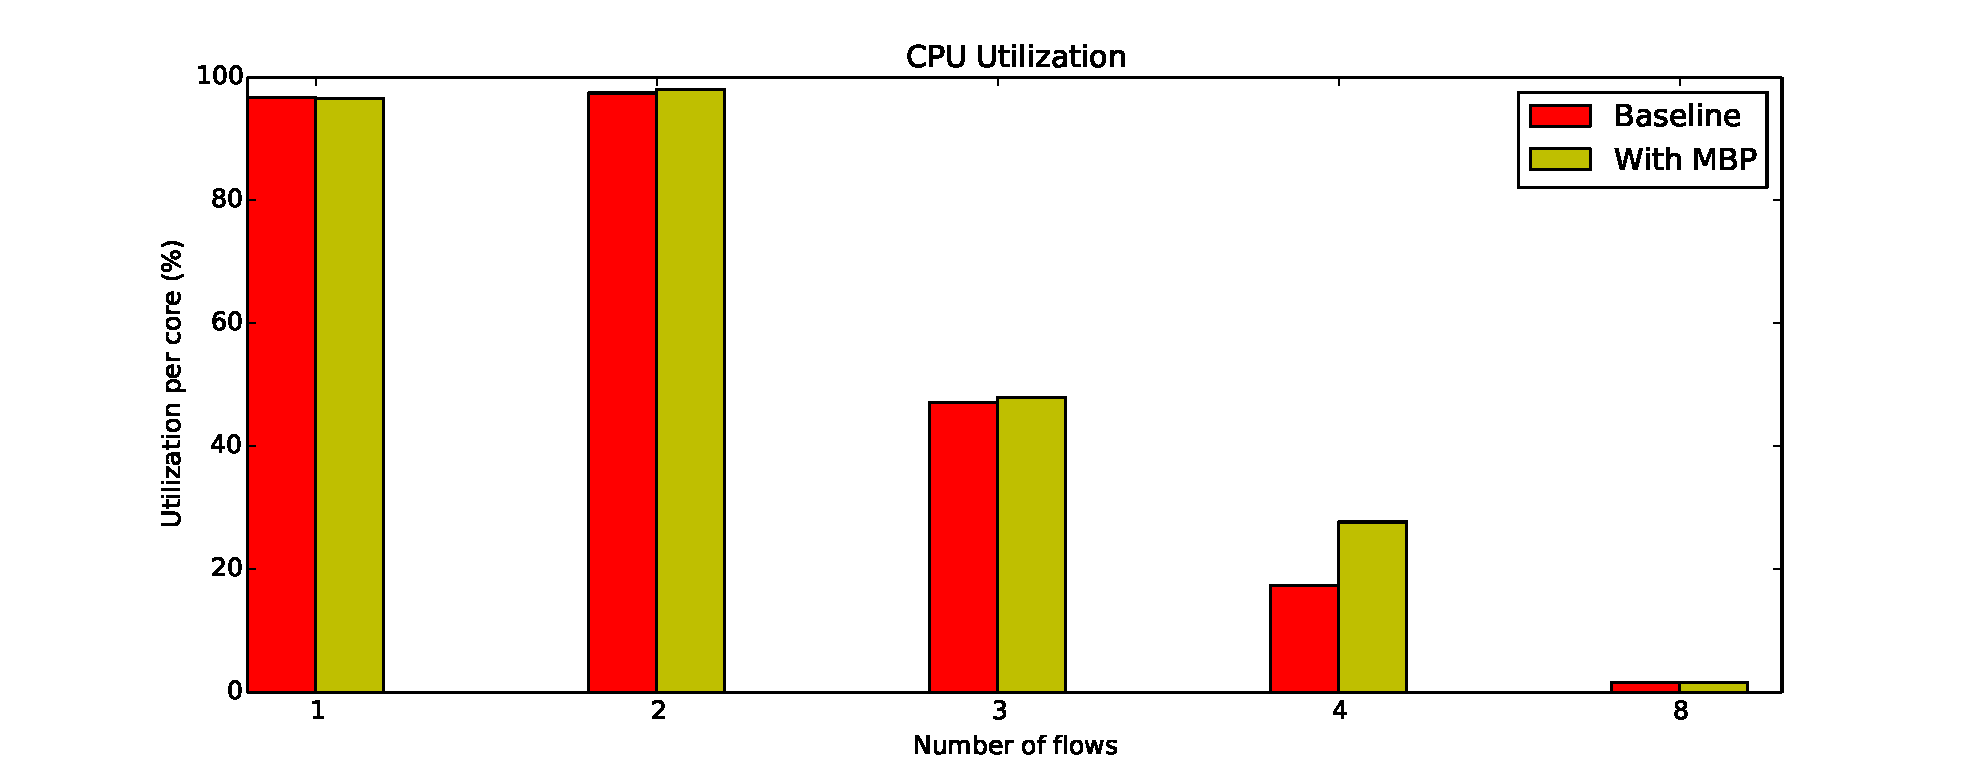
\includegraphics[width=\linewidth]{figures/CPU.pdf} 
% 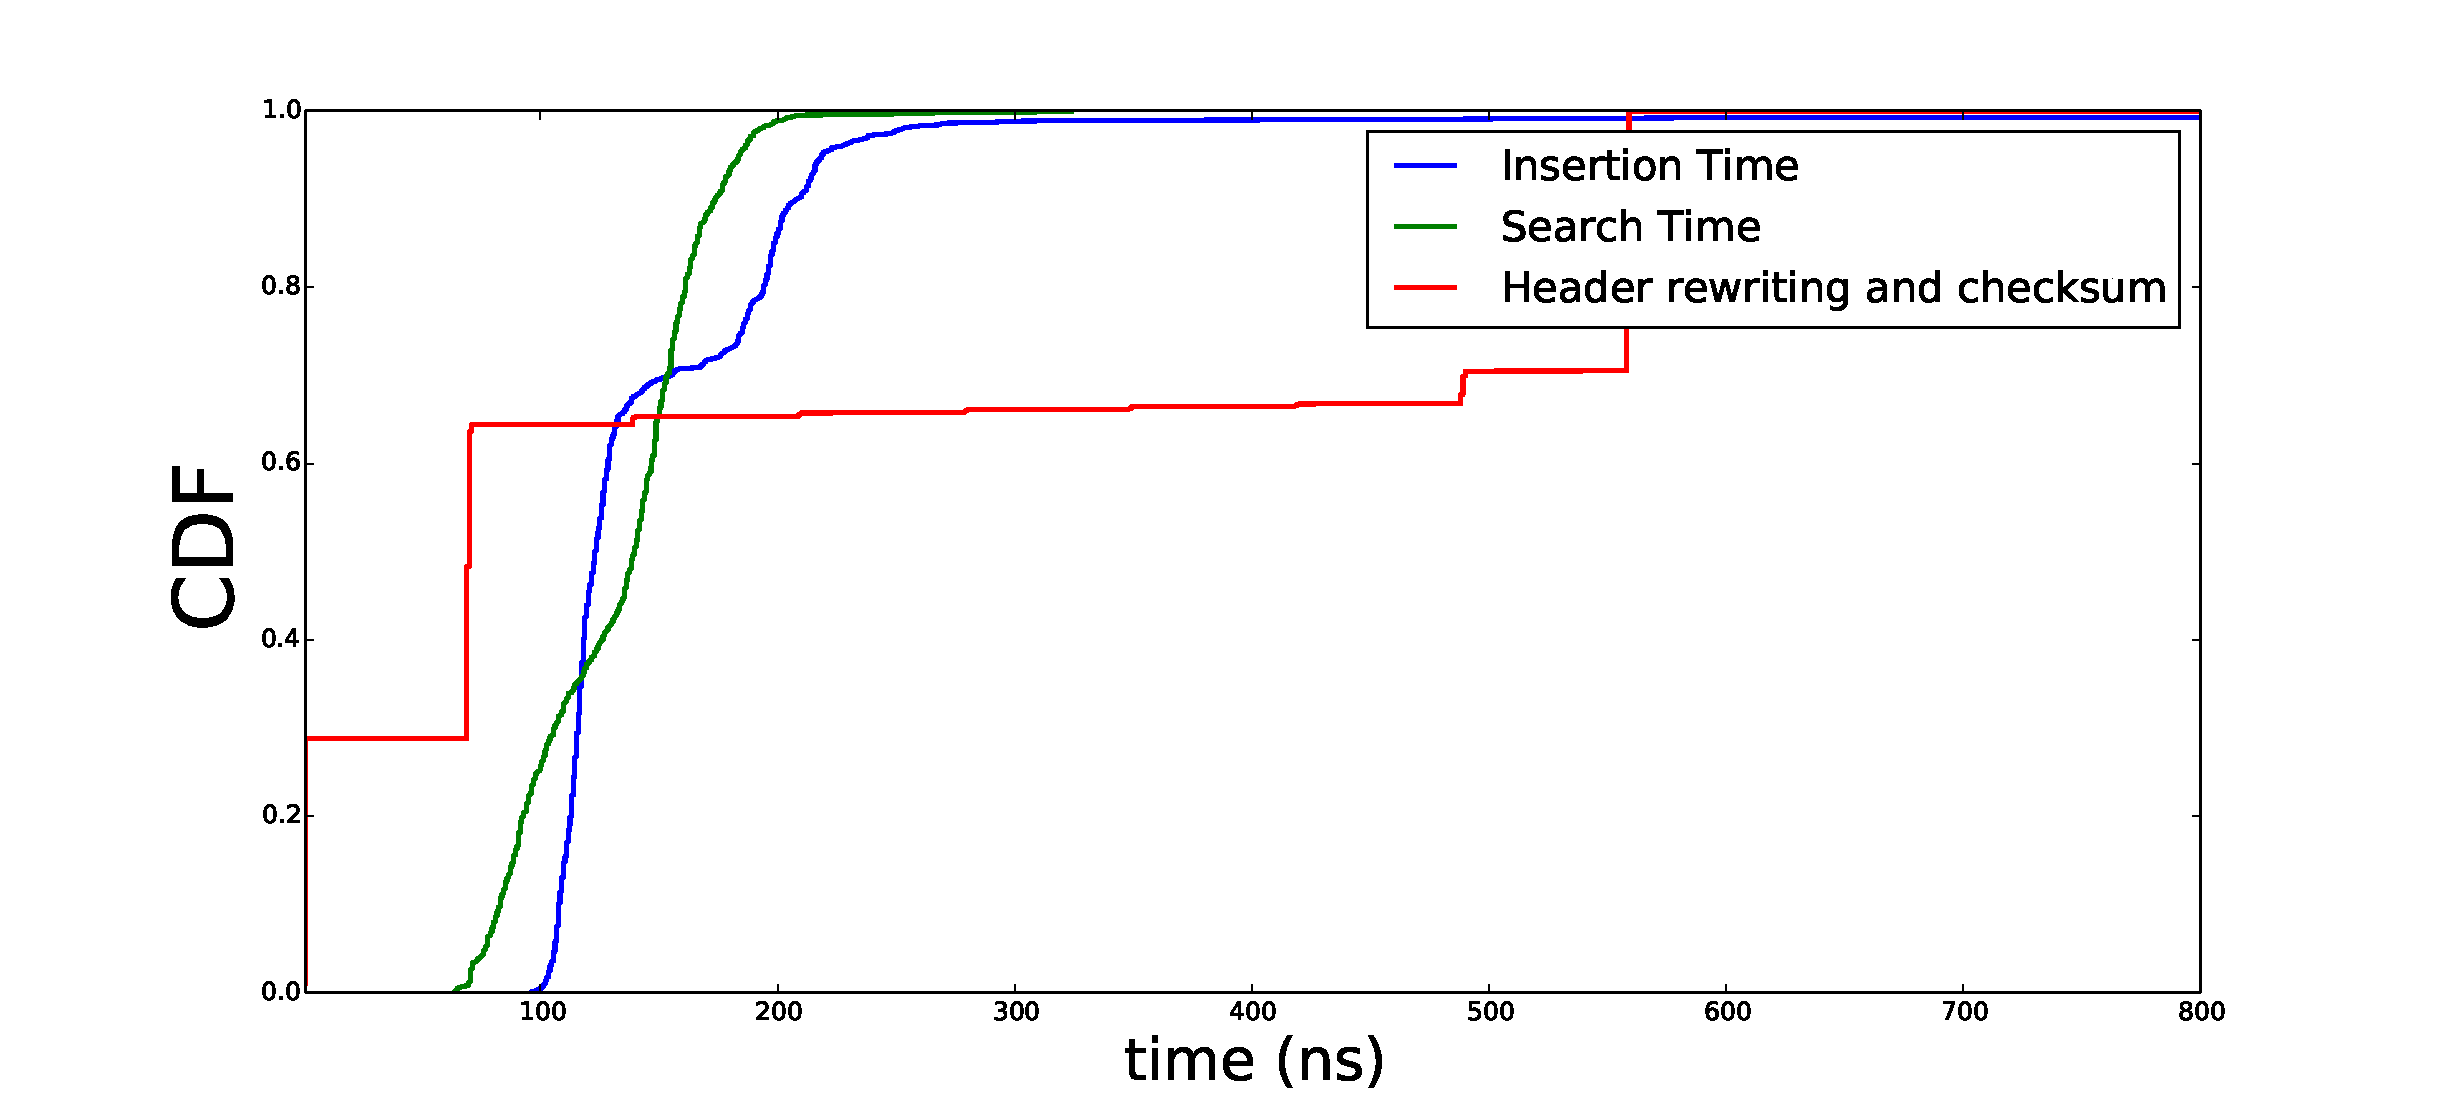
\includegraphics[width=\linewidth]{figures/cdf.pdf} 
\caption{\small Average CPU utilization in stress test. Note we only include the cores that are interrupted by the NIC.}\label{throughput}
\end{figure}

We plotted the CPU utilization of the middlebox in the same experiments. Note since the middlebox acts as a software router without the kernel module, it also consumes a certain amount of CPU cycles. The highest difference between the baseline and the system lies in the setting of 4 flows, the utilization is 10\% higher than that of the vanilla system (27.6\% versus 17.2\%), but under most circumstances the gap is within 2\%. One thing worth noting is that as the number of flow increases, the CPU utilization per core plummets, our explanation is that since the testbed machine has 16 cores and 32 hyper-threads, it spreads out quite evenly, and the CPU utilization scales linearly at high load but it is not the case at low load (e.g., 1M packets/s causes much higher CPU utilization than 500K packets/s). 


The experimental result is promising and proves that the in-kernel data plane implementation can offer very high throughput at the cost of modest increase of CPU utilization. 



\subsection{Latency}
We evaluate our system's latency in the following order: (i) how much overhead it has for a super-session setup? (ii) how much overhead it has during loss-free, packet order-preserving, and substream separation and order preserving update, even in the case of data packet loss or reordering. 


\subsubsection{Three-Way handshake}
% \kelvin{will add more stuff, like three hops, 4 hops and 5 hops, but do get the idea of how to do it now, three hops values are 426.5 28.7515216989, 464.5 22.8527897641, 688.1 24.6473122267}
We first measure the latency for session establishment, in a topology of three hops (client - middlebox - server). We have two different implementation, (i) out of band UDP ahead to TCP handshake, (ii) piggyback TCP handshake at the payload. Not surprisingly, TCP piggyback can greatly reduce the extra latency due to propagation delay, with a modest increase less than $40 \mu $s. On the other hand, out-of-band UDP incurs $688\mu$s delay ahead of TCP handshake. 

\begin{figure}[ht]
\centering
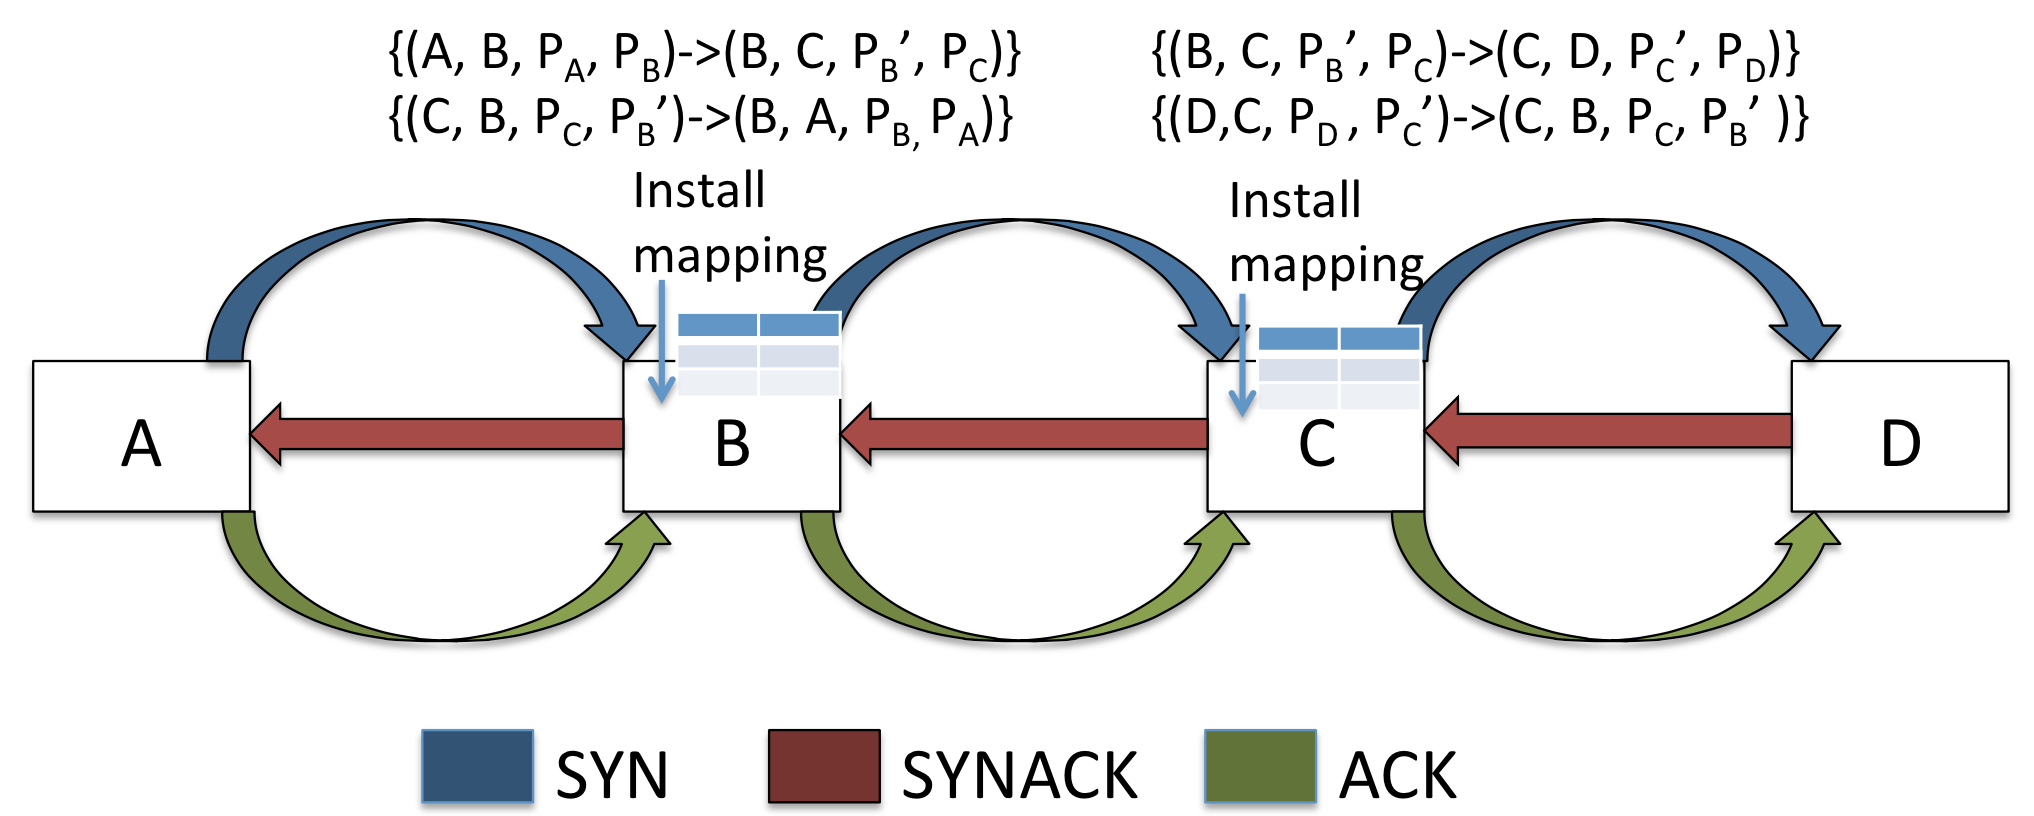
\includegraphics[width=\linewidth]{figures/threeway.png} 
\caption{\small Latency for session establishment}\label{threeway}
\end{figure}
\subsubsection{Flow Migration}
\system supports flow migrations with various properties. We also measure the time interval for a loss-free, order-preserving, and byte stream order preserving update.   

We run our experiments in a topology with four middleboxes (A,B,C,D), there are two paths (A-B-D) and (A-C-D) that each consists of three middleboxes. The goal of the flow migration is to replace middlebox B with D. We measure the latency for such migration, using (a) loss-free migration, (b) order-preserving migration, and (c) (a different property). The latency are evaluated under different loads on a network with all 1Gbps links. 

As shown in the table, we can see that not surprisingly, as the load of the network increases, the update latency increases. We attribute the increase to two causes, the queuing delay in the network and the scheduling delay in local servers. In loss-free migration, the old path is saturated; however, the new path is idle and thus the increase is due to the high load in server. In order-preserving migration, the update is on hold until both the new and old paths have sent notification, and thus the queuing delay also contributes to the latency. 

\begin{table}[ht]
\centering
\small
\begin{tabular} {|c |c | c| c|}

\hline
Load&Loss-Free& Order-Preserving\\ \hline 

\textbf{0\% }  &1.7ms & 2.3ms \\ \hline
\textbf{50\% }  & 2.1ms &2.6ms \\ \hline
\textbf{100\% }  & 3.6ms &14ms \\ \hline

\end{tabular}
\caption{Flow migration update time under different network load} \label{movelatency} 
\end{table}

The results demonstrate that the system can deal with flow migrations in the order of tens of milliseconds. To put in perspective, the time for a middlebox state migration is above 100ms~\cite{splitmerge, OpenNF} and a fast consistent update takes up to a second~\cite{xinjin}, a more detailed breakdown is in table~\ref{latencycomp}.

\begin{table}[ht]
\centering
\small
\begin{tabular} {|c |c | c| c|}

\hline
 &Loss-Free& Order-Preserving \\ \hline 
% &~\cite{SIMPLE,FLOWTAGS, OpenNF}& ~\cite{CoMB, splitmerge}& ~\cite{ Aplomb,DOA,I3} & ~\cite{OVS, Netfilter} & \\ \hline

Split/Merge
\footnote{\scriptsize at packet rate 37.5 kpps, time are consumed across flow migration and state migration} 
		&~500ms&$\otimes$\footnote{\small not supported} \\ \hline
OpenNF(a)
\footnote{\scriptsize flow update time at packet rate 2.5-10 kpps, (a) is for flow migration time, and (b) is for middlebox state migration time} 
	       & 84ms& 96ms\\ \hline
OpenNF(b)      & 134ms& 208ms \\ \hline
Dionysus
\footnote{\scriptsize Large scale networks}
	      &600-1200ms &$\otimes$  \\ \hline
Our system
\footnote{\scriptsize at packet rate 75 kpps (900 Mbps)} 
	    & 4ms &14ms \\ \hline

\end{tabular}
\caption{Comparison with other dynamic middlebox and flow migration systems}\label{latencycomp} 
\end{table}



\section{Discussion}
\label{sec:discussion}

incremental deployment

security

fault tolerance





%%%%%%%%%%%%%%%%%%%%%%%%%%%%%%
%%%%%Related work
%%%%%%%%%%%%%%%%%%%%%%%%%%%%%%
%%%%Comparison table %%%%%%%%%

\begin{table*}[ht]\label{compare} 
\centering
\small 

\begin{tabular} {l |c | c| c| c| c }


                            			     &Scalable Fine-              &   Low Performance    &  NF's  Flow      &  Host        &  Incremental \\
						     &Grained NF Policy    	  &   Overhead           & Migration       &  Mobility   & Deployment \\\hline
						     
NF Policy                                           & TCAM size,      	          &                      & not discussed      &   not discussed  & inter-domain  \\
Enforcing~\cite{SIMPLE,FLOWTAGS}                   & TCAM update speed          &                      &                   &               &  middlebox \\ \hline


NF Dynamic                                          &TCAM size,     	          &  Handle packets      &                &  not discussed    & inter-domain\\ 
Control~\cite{OpenNF,splitmerge}                       &  TCAM update speed         & at the controller     &                &                & middlebox  \\   \hline


Naming service                          &			  	 & VPN, or per packet encap-                   & not discussed       & not discussed &  [some] new naming system  \\ 
based~\cite{DOA, Aplomb}                         &                              & sulate and identify          &                    &                  & new socket abstraction     \\\hline 



\end{tabular}
\caption{\small Reasons that different NF policy steering and mobility solutions failed to fulfill the properties}
\end{table*}





\section{Related work}

\textbf{Middlebox in SDN:}
SIMPLE~\cite{SIMPLE} and FlowTags~\cite{FLOWTAGS} take advantage of the switches with a fine-grained rule support in software-defined network (SDN), and support network function policy chaining in traditional and NFV setting respectively. Both approaches are constrained by the TCAM size, a hardware limitation in terms of fine-grained policy, and neither not support NF migration or host mobility. 

OpenNF~\cite{OpenNF} and Split- Merge~\cite{splitmerge} leverage the SDN controller to manage NF's state migration and NF's flow migration. However, since the central controller is involved in both control plane (update the network rules) and data plane (buffer the packets on the fly during migration), they suffer from high latency and low scalability. They also suffer from hardware limitation for fine-grained policies.  

\textbf{Middlebox using naming service:}
DoA~\cite{DOA} uses a delegation-oriented global naming space architecture, that explicitly specifies intermediary middleboxes on the path. Two key distinction between DoA and \system is that (i) \system does not require any new naming service and (ii) DoA does not support dynamic policy service. APLOMB~\cite{Aplomb} outsources the network functions to the cloud with a naming service indirection. It uses VPN to tunnel the traffic to the cloud and use DNS-based indirection to decide which cloud to enforce the middlebox policy. It assumes the cloud can provide elastic NF service but it cannot explicitly handle dynamic policy chain. 


\textbf{Middlebox consolidation:}
CoMB~\cite{COMB} and click~\cite{ClickOS, click} both consolidate network functions as an application or a VM image, and one host machine can run multiple instances of different network functions. Both approaches are mainly focused a feasibility and scalability of network functions on a single generalized servers. Both solutions consider neither scale-out across servers nor NF and flow migration.

\textbf{Mobility Protocols:}
Mobility protocols use (i) a fixed indirection point (e.g., Mobile IP~\cite{mip}), (ii) redirecting through DNS (e.g., TCP Migrate~\cite{TCPMobile}), (iii) indirection infrastructure (e.g., ROAM~\cite{I3Mobile}) or (iv) indirection at the link layer (e.g., cellular mobility). None of them consider the existence of middleboxes. Coexistence of network functions and new protocols is especially important for deployment, as a study in multipath TCP shows~\cite{MPTCP}. \system shares some similarity with many mobility protocols and has support for network functions.   

\small
\bibliographystyle{acm}

\bibliography{ref}

\end{document}
